\chapter{Úvod}

Od jednoduchých začiatkov hier s textom a ASCII grafikou sa dnes vyvinuli do hyperrealistických diel. Toto miliardové odvetvie je ako obrovský, dynamický organizmus, ktorý sa neustále mení, vyvíja a prispôsobuje. Menší vývojári hier majú v súčasnosti v tomto odvetví viac príležitostí vďaka platformám, ako je Steam, ktoré toto odvetvie výrazne otvorili verejnosti. V súčasnosti už nie je potrebné mať veľké štúdio a marketingový rozpočet na vydanie hry. Aj keď menšie štúdiá nemusia mať toľko zamestnancov ako ich väčší konkurenti, trh sa od zavedenia technológie procedurálneho generovania (ďalej PCG) stal rovnejší. Menšie tímy teraz môžu vďaka tejto inovácii vytvárať obstojné herné tituly a uživiť sa na trhu plnom veľkých korporátnych značiek.

V záujme udržania záujmu hráčov, v dnešnom rýchlom svete, pridáva PCG hrám predovšetkým rozmanitosť a nepredvídateľný prvok. Poskytnutím jedinečného zážitku pri každom hraní, zvyšujeme hodnotu aj znovuhrateľnosť hry. A to je obzvlášť dôležité na trhu, kde existuje neustála a tvrdá konkurencia v boji o hráčov.

PCG tiež pomáha vývojárom spravovať ich zdroje. Vývoj hier môže byť náročný na ľudský kapitál, časovú náročnosť a financovanie, pretože mnohé úrovne a zložité prostredia sa vytvárajú ručne. Využitím algoritmov pre ich tvorenie a automatizovaním niektorých prvkov hry, tak znížime výrobné náklady a časové lehoty. V odvetví, kde môže byť čas uvedenia na trh rozhodujúcim faktorom úspechu, je táto efektivita na nezaplatenie. PCG je teda nástroj používaný pri vývoji hier na podporu efektívnosti a kreativity. Umožňuje vytvárať rozsiahle, rozmanité a~pútavé herné svety, čo je v súlade s neustálym úsilím tohto odvetvia o~inovácie a~zlepšovanie zážitku hráčov.

Generovanie máp vo videohrách sa začalo v začiatkoch tohto odvetvia a vyvinulo sa od jednoduchých, ručne kreslených návrhov, až po komplexné, algoritmicky generované prostredia. Bola to koncepčná aj technologická revolúcia, pričom tituly ako Rogue a Elite, pôsobili ako priekopníci a vystavili hráčov doposiaľ neprebádaným prostrediam, ktoré boli pri každom hraní unikátne vytvorené od základu.

Hlavným predmetom tejto práce je dôkladná analýza metód PCG, konkrétne metód používaných na tvorbu 2D máp vo videohrách. Cieľom je rozobrať a preskúmať rôzne prístupy, zhodnotiť ako dobre fungujú v rôznych herných prostrediach a implementovať jednotlivé metódy generovania v jednoduchej hre.

\label{sec:theory}
\chapter{Teória} % Teoretická časť 

Procedural Content Generation (ďalej PCG) je dnes široko používanou technikou v neustále sa meniacom priemysle videohier. Vo svojej podstate ide o algoritmické generovanie herného obsahu. Príkladom tohto typu obsahu sú textúry, mapy, herné úrovne aj príbehové komponenty. Výhodou je schopnosť vytvárať originálne herné zážitky a súčasne odbremeniť ľudských vývojárov, skrátiť celkový čas na vývoj hier a znížiť tým náklady.

Počiatky PCG možno nájsť v hrách ako Rogue\footnote{Článok Rogue 1980 - \url{http://pcg.wikidot.com/pcg-games:rogue}}. Kde bola technika najprv vyvinutá ako riešenie tvorenia neobmedzeného počtu máp. Dnes nachádza využitie aj mimo generovanie máp a to napríklad pri grafike ako uvádza Ebert, D. S. vo svojej knihe Textúrovania a~modelovania \cite{ebert2003texturing}. Ďalším využitím môže byť generovanie nepriateľov ako uvádzajú Pereira a~kol. v správe SBGames \cite{pereira2021procedural}. A nájdeme aj princípy generovania príbehových prvkov, ktoré popisuje práca Young a kol. \cite{young2013plans}.

PCG tak uľahčuje prácu pre veľké štúdiá, ale aj nezávislým vývojárom. Ktorých v poslednej dobe pribúda čoraz viac, ako uvádza Herd vo svojom článku \footnote{Článok Forbes - \url{bit.ly/4a5NO7T}}. Využitie PCG a stále napredujúcej umelej inteligencie znamená zmenu v spôsobe, akým sa vytvárajú herné svety. Hry teraz môžu prekročiť hranice vopred ručne pripraveného obsahu a poskytnúť používateľom originálny zážitok pri každom hraní.

V tejto kapitole sa hlbšie pozrieme sa na jeho početné využitie pri navrhovaní hier, pričom sa zameriame na generovanie 2D máp. Cieľom tohoto skúmania je prehľad a analýza najrôznejších metód, ich možnosti a nedostatky. V závere kapitoly sa budeme venovať algoritmom potrebným pre vyhľadávanie cesty, ktoré využijeme neskôr v našej hre.

\section{Prehľad metód} 

Do tabuľky \ref{tab:function-table} sme pripravili prehľad najčastejšie sa vyskytujúcich metód generovania máp. Pretože v praxi herné štúdiá často používajú komplexné využitie týchto metód, uvádzanie príkladov jednotlivých hier je až na pár výnimok čisto orientačné a slúži pre predstavu, čoho je daná metód sama o sebe schopná generovať. Ďalej si prejdeme jednotlivé metódy samostatne a pozrieme sa na ne viac do hĺbky. Začneme metódami generujúcimi mapy alebo miestnosti a následne prejdeme metódami, ktoré sa dajú použiť na prepojenie jednotlivých častí máp. Nakoniec predstavíme uplatnenie PCG na vkladanie nepriateľov a objektov do mapy.

\begin{table}[H] \label{table}
    \centering
    \begin{tabular}{|m{5em}|m{13em}|m{11em}|m{6em}|}
      \hline
      \textbf{Metóda} & \textbf{Parametre a kontrola} & \textbf{Najlepšie využitie} & \textbf{Výsledok} \\ 
      \hline
      Binary\newline Space\newline Partitioning & Pomery\,rozdelenia,\,veľkosť \newline miestností,\,pravidlá\,spájania & Generovanie neprekrývajúcich sa miestností & Doom\tablefootnote{Článok Doom - \url{https://twobithistory.org/2019/11/06/doom-bsp.html}} \\
      \hline
      Cellular\newline Automata & Pravidlá\,susediacich\,buniek, \newline počiatočný\,stav,\,počet\,iterácií & Komplexné jaskynné\newline štruktúry & Terraria, Dwarf\newline Fortress \\
      \hline
      Diamond Square & Drsnosť,\,počiatočné\,rohové\newline hodnoty & Realistické\,výškové\,mapy\newline terénu & SimCity \\
      \hline
      Diffusion\newline Limited\newline Aggregation & Pravidlá pohybu častíc,\newline pravdepodobnosť prilepenia & Prirodzené vzory rastu,\newline snehových vločiek & Core\newline Keeper \\
      \hline
      L-systems & Súbory pravidiel, počiatočný\newline axióm, počet iterácií & Organické štruktúry ako\newline stromy, jaskynné systémy & Spelunky \\
      \hline
      Perlin\newline Noise & Frekvencia, amplitúda,\newline oktávy & Prirodzene vyzerajúci\newline terén krajiny & Minecraft,\newline Terraria \\
      \hline
      Random\newline Room\newline Placement & Veľkosť miestností, rozostup,\newline pravidlá spájania & Náhodné rozloženie\newline dungeonov & Binding of\newline Isaac\tablefootnote{Článok Binding of Isaac - \url{bit.ly/4b1XP7B}} \\
      \hline
      Random\newline Walk & Dĺžka\,kroku,\,pravdepodobnosť\newline smeru & Vytváranie ciest a riek & Don't\newline Starve \\
      \hline
      Voronoi\newline Diagrams & Počiatočné\,body,\,metriky\newline vzdialenosti & Rozdelenie regiónov,\newline biomov & Core\,Keeper\tablefootnote{Článok Core Keeper - \url{https://corekeeper.atma.gg/en/World}} \\
      \hline
      Wave\newline Function\newline Collapse & Súbor dlaždíc, pravidlá\newline priľahlosti & Náhodné\,rozloženie~dungeonov & Bad\,North\,\cite{nordvig2020expanding}  Townscaper\tablefootnote{Článok Townscaper - \url{bit.ly/44uXqb4}} \\
      \hline
    \end{tabular}
    \caption{Metódy PCG pre 2D svety}
    \label{tab:function-table}
\end{table}

\section{Binary Space Partitioning} \label{sec:bsp}

V procedurálnom generovaní je binárne rozdeľovanie priestoru (ďalej BSP), technika používaná na delenie veľkého celku (napríklad veľkosť mapy celej úrovne hry) na diskrétne oblasti. Funguje na princípe výberu oblasti, ktorú rekurzívne rozdeľuje na polovice striedaním vodorovných a zvislých rezov kým nedosiahneme vopred definovanú minimálnu veľkosť. Tento proces (viď obr. \ref{fig:bsp-proces}) vytvára stromovú štruktúru (viď obr. \ref{fig:bsp-tree}), v ktorej každý uzol znamená časť priestoru.

BSP je obzvlášť užitočný na vytváranie náhodných, ale štruktúrovaných herných oblastí ako sú miestností dungeonov. Uľahčuje efektívnu organizáciu herného priestoru a zaručuje, že úrovne sú prestupné. Táto metóda dobre funguje v hrách, kde sú rozloženie úrovní a~spôsob ich vzájomného umiestnenia dôležitými aspektmi hrateľnosti \cite{putra2023bsp}. 

Aj keď samotná metóda neponúka spôsob prepojenia jednotlivých celkov, vhodným spôsobom ju vieme rozšíriť o algoritmy ktoré sa o prepojenie miestností postarajú. Pri použití tejto metódy máme k dispozícii pomer rozdelenia, minimálnu veľkosť miestnosti, možnosť pridať odsadenie medzi miestnosťami a pravidlá spájania ako kontrolné parametre ktorými vieme ovládať výslednú mapu. Výhodou tejto metódy je záruka neprekrývania sa miestností. A pri spájaní miestností podľa najbližšieho stredu vieme zaručiť aj lineárnu náväznosť levelu.

\begin{figure}[H]
    \centering
    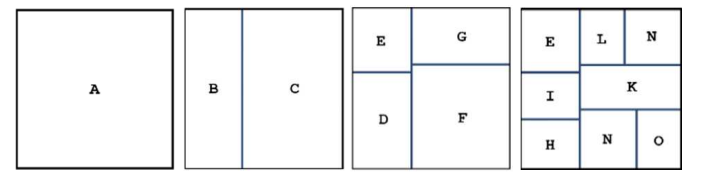
\includegraphics[width=0.5\linewidth]{obrazky-figures/bsp-squares.png}
    \caption{Postup procesu rozdeľovania plochy v smere zľava, doprava \cite{putra2023bsp}}
    \label{fig:bsp-proces}
\end{figure}

\begin{figure}[H]
    \centering
    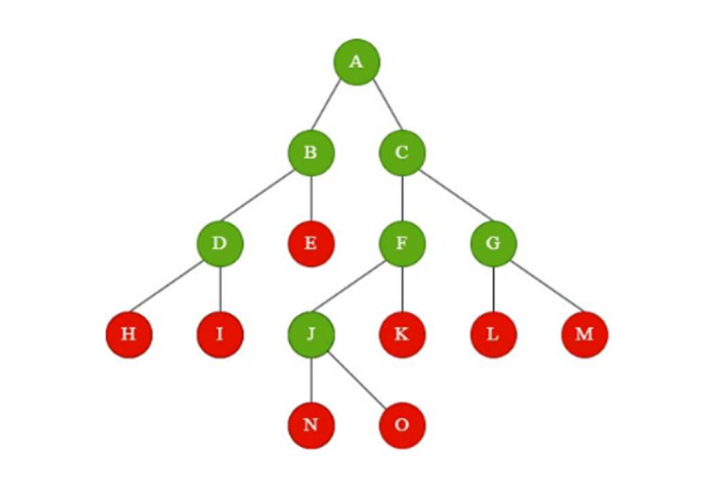
\includegraphics[width=0.5\linewidth]{obrazky-figures/bsp-tree.png}
    \caption{Vizualizácia stromovej štruktúry výsledného rozdelenia \cite{putra2023bsp}}
    \label{fig:bsp-tree}
\end{figure}

\section{Bunkové Automaty} \label{sec:ca}

Bunkové automaty (z angl. Cellular Automata, ďalej len CA) sa okrem simulačného použitia využívajú aj v hernom vývoji. Podľa definície za CA považujeme matematické reprezentovanie zložitých prírodných systémov, zložených z jednoduchých a rovnakých komponentov, ktoré na seba lokálne pôsobia. Skladajú sa z mriežky, pričom každá ma obmedzený rozsah možných hodnôt. Všetky hodnoty sa vyvíjajú synchrónne v diskrétnych časových krokoch a podľa rovnakých pravidiel. Daná hodnota v danom kroku sa určí podľa hodnôt v jeho okolí (viď obr. \ref{fig:ca-neighbours}) počas predchádzajúceho kroku (viď obr. \ref{fig:ca-iterations}) \cite{wolfram1984universality}.

\begin{figure}[H]
    \centering
    \begin{minipage}[c]{0.45\linewidth}
        \centering
        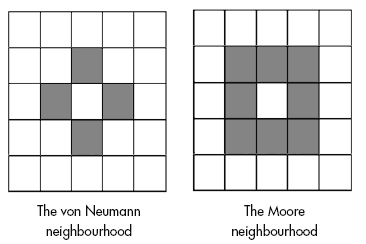
\includegraphics[width=0.8\linewidth]{obrazky-figures/ca-neighbourhood.png}
        \caption{Často používané okolia bodov}
        \label{fig:ca-neighbours}
    \end{minipage}
    \hfill
    \begin{minipage}[c]{0.45\linewidth}
        \centering
        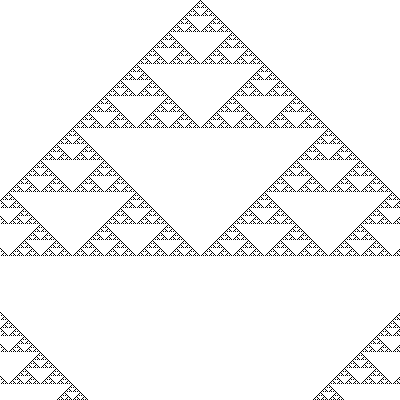
\includegraphics[width=0.6\linewidth]{obrazky-figures/ca-pattern.png}
        \caption{Príklad iterovania 1D automatu zhora nadol}
        \label{fig:ca-iterations}
    \end{minipage}
\end{figure}

Keďže táto technika dokáže napodobniť organické procesy, v PCG sa najčastejšie využíva pri vytváraní prírodných štruktúr, ktoré majú mať realistický vzhľad ako napríklad jaskynný systém, močiare a ostrovy. Vďaka svojej flexibilite sa CA môže používať so širokou škálou nastavení, čím sa vytvárajú dynamické a rozmanité herné svety.

Metóda môže mať využitie pri generovaní jednotlivých miestností na predom určených miestach, bludísk \cite{adams2017cellular}, no jej najväčší potenciál je v generovaní celých máp, alebo úsekov jaskýň, ktoré na seba nadväzujú. Táto technika nám dáva niekoľko kontrolných parametrov ktorými ovplyvňujeme výsledok, sú to pravidlá okolia susedov, veľkosť okolia, počiatočný stav mriežky a počet iterácií. Pre potreby našej práce sa zameriame na 2D mriežku s~Moorovym okolím a budeme experimentovať s rôznymi nastaveniami.

\section{Diamond-Square}

Jedna z ďalších techník na vytváranie realistických výškových máp krajiny v 3D, je algoritmus diamantového štvorca (ďalej DS). Miller Gavin S. P. ho vo svojej práci definuje ako proces vytvárania fraktálnych vzorov náhodným posunom stredných hodnôt mriežky, prostredníctvom opakovaného delenia \cite{miller1986diamonsquare}. Táto metóda vyniká pri vytváraní výškových máp v 3D, pretože napodobňuje prirodzené kolísanie terénu. Navyše na rozdiel od iných generovaní výškových máp pomocou šumu je táto metóda rýchlejšia \cite{rose2016brief-diamondsquare}.

Pri tejto metóde začíname so štvorcovou mriežkou, s typickou veľkosťou podľa rovnice x rovné 2 na n-tú mocninu plus 1, kde za \textit{n} dosadzujeme celé kladné číslo. Následne sa inicializujú rohové body s náhodnou hodnotou. Hodnoty v bodoch predstavujú ich výšku. Následne sa striedavo aplikujú pravidlá diamantového a štvorcového kroku (viď obr. \ref{fig:ds-steps}) než sa vyplní celá mriežka novými hodnotami. Je pri tom dôležité aby sa pravidlá aplikovali v správnom poradí, výsledok vieme kontrolovať drsnosťou teda v akých krokoch znižujeme umelo pridávanú hodnotu a počiatočnými hodnotami rohových bodov.

\begin{enumerate}
    \item Diamantový krok - Nájde stredový bod štvorca medzi rohovými bodmi. Vypočítame novú hodnotu pre tento stred ako priemer rohových bodov a pridáme k nemu náhodnú hodnotu. (Náhodná hodnota vnáša premenlivosť a zvyčajne sa pri každej iterácii znižuje, aby sa zabezpečil hladší terén v detailnejších mriežkach.) Výsledkom je kosoštvorec na ktorí aplikujeme štvorcový krok
    \item Štvorcový krok - Vypočíta výšky stredových bodov každej hrany štvorca. Tieto body sa vypočítajú ako priemer dvoch rohových bodov danej hrany a najbližšieho stredového bodu z diamantového kroku a pripočítame náhodnú hodnotu pre variabilitu. Výsledok sú menšie štvorce v každom kvadrante pôvodného štvorca.  
\end{enumerate}

Tieto pravidlá sa opakovane aplikujú na každý z menších štvorcov a kosoštvorcov.

\begin{figure}[H]
    \centering
    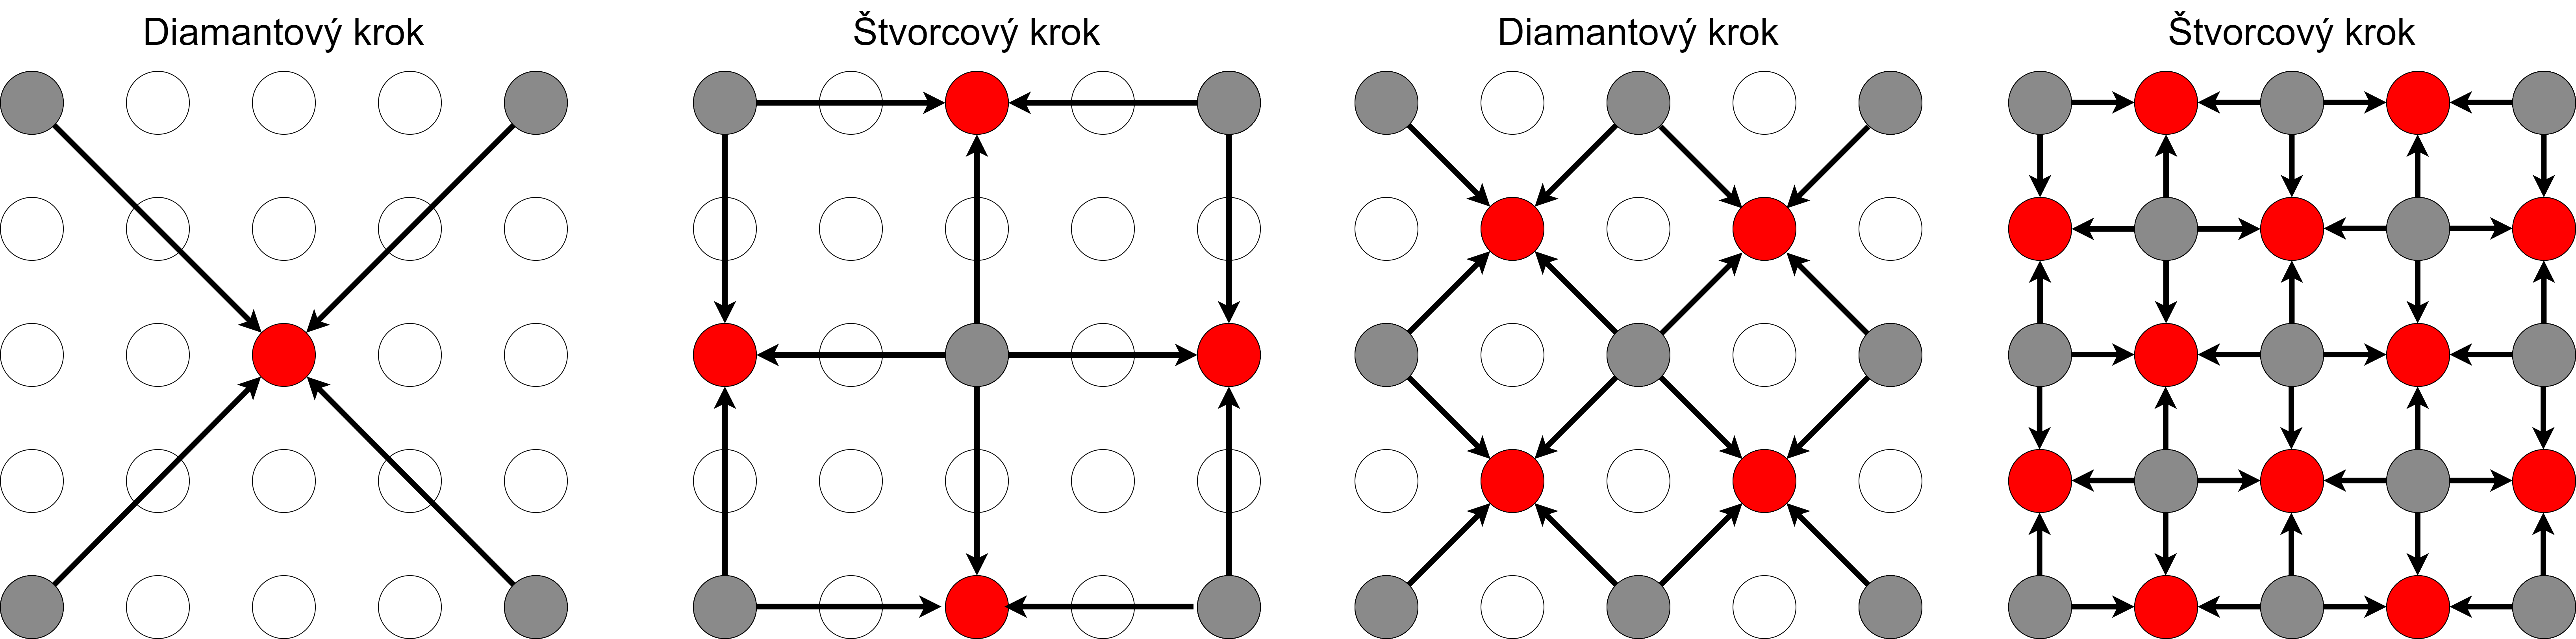
\includegraphics[width=0.75\linewidth]{obrazky-figures/ds-iteration.png}
    \caption{Ukážka fungovania DS algoritmu na mriežke o veľkosti 5x5}
    \label{fig:ds-steps}
\end{figure}

\section{Diffusion-Limited Aggregation}

Agregáciu obmedzenú difúziou (ďalej DLA) vieme podľa práce Witten T. A. Jr. a Sander L. M. chápať ako proces tvorby zhlukov, pri ktorom sa častice prilepia k rastúcej štruktúre prostredníctvom náhodného pohybu \cite{witten1981diffusion}. Vo vedeckom odvetví sa pre tento pohyb používa Brownov pohyb\footnote{Teória Brownovho pohybu - \url{https://journals.aps.org/pr/abstract/10.1103/PhysRev.36.823}}. Pre naše potreby nám postačí pseudonáhodný pohyb, simulovaný metódou Random Walk (viď kapitola \ref{random-walk}). Tento proces sa dá napríklad využiť pri modelovaní minerálnych ložísk alebo snehových vločiek (viď obr. \ref{fig:dla}).

V PCG môže napodobňovať rastové procesy a tvorbu fraktálnych vzorov. Takéto vzorce sú prirodzenejšie a dajú sa využiť na generovanie riek alebo jaskýň ako ukazuje jeden z~článkov Noveltechu\footnote{Článok DLA, Noveltech - \url{https://www.noveltech.dev/unity-procgen-diffusion-aggregation}}. Výsledok metódy vieme kontrolovať zmenou pravidiel pohybu a~pravdepodobnosťou prilepenia častíc. Výraznú zmenu výsledkov vieme spôsobiť pridaním príťažlivej sily, kedy častice pohybujúce sa v systéme budú ovplyvňované pri výbere smeru pohybu, smerom k bodu príťažlivej sily. Najčastejšie ide o bod v centre mapy. Takto zmenená metóda sa nazýva DLA s centrálnym bodom príťažlivosti (DLA with Central-Attractor)\footnote{Článok DLA, Bourke, P.  - \url{https://paulbourke.net/fractals/dla/}}.

Samotný proces pozostáva z piatich krokov:

\begin{enumerate}
    \item Inicializácia - Začneme vytvorením základného bodu, ktoré bude základným semienkom
    \item Vytvorenie častice - Vyberieme náhodný bod kdekoľvek na mape
    \item Náhodný krok - Častica sa náhodne pohybuje po mape (Brownov pohyb, resp. Random Walk)
    \item Agregácia - Ak sa častica dotkne semienka alebo už agregovanej častice, prilepí sa a~stane sa súčasťou zhluku
    \item Opakovanie - Krokmi 2 až 4 pridávame nové častice 
\end{enumerate}

\begin{figure}[H]
    \centering
    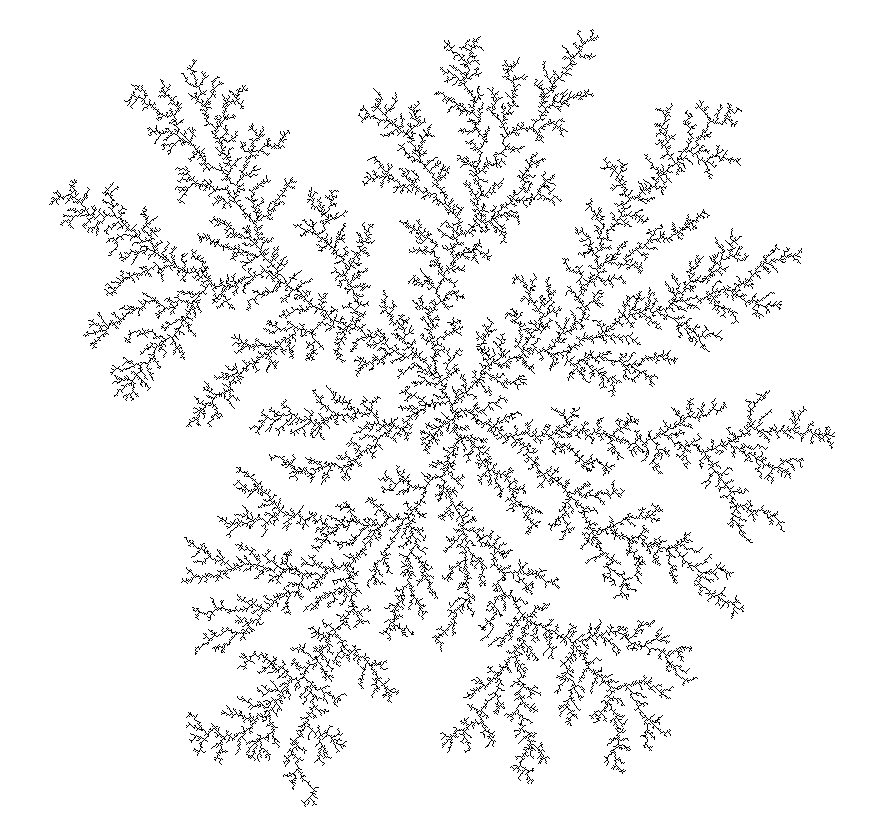
\includegraphics[width=0.4\linewidth]{obrazky-figures/dla-graph.png}
    \caption{Príklad výstupu metódy DLA pre formovanie snehových vločiek}
    \label{fig:dla}
\end{figure}

\section{Formálne Gramatiky}

Podľa práce o formálnej jazykovej teórii od Jäger, G. a Rogers, J., považujeme za formálny jazyk množinu reťazcov alebo sekvencií nad určitým konečným slovníkom. Takýto slovník sa pri aplikovaní na prirodzení jazyk stotožňuje so slovami, morfémami alebo zvukmi \cite{jager2012formal}. V našej práci sa zameriame na samotné gramatiky, ich pravidlá a ako sa dá využiť formálny jazyk, ktorý popisujú, pre generovanie v hernom priemysle.

Metódy budú používať formálnu gramatiku pozostávajúcu z abecedy symbolov, pravidiel transformácie nad touto abecedou a pre začiatok generovania aj počiatočný reťazec. Následným iterovaním nad týmto reťazcom ho podľa pravidiel rozširujeme a transformuje ľubovoľný počet krát. Týmto procesom vieme vytvoriť geometrické štruktúry a ich tvar kontrolujeme zmenou pravidiel alebo počiatočného reťazca.

V praxi nájdeme niekoľko rôznych metód ktoré pracujú s iným druhom gramatiky. Bližšie sa pozrieme na L-systémy a Generatívne gramatiky, no za zmienku stoja aj grafové\footnote{Vedecký článok - \href{https://www.researchgate.net/publication/239580441_Handbook_of_Graph_Grammars_and_Computing_by_Graph_Transformation}{Príručka grafových gramatík a výpočtov pomocou transformácie grafov}} a priestorové/tvarové gramatiky\footnote{Práca - \href{https://citeseerx.ist.psu.edu/document?repid=rep1\&type=pdf\&doi=6dc9c55dade136193780a3ce0f5269036c5127cf}{Tvarové gramatiky a generatívna špecifikácia maľby a sochy}}, využívané na generovanie misií a priestoru ako ukazuje práca o level dizajne od Dormans, J. \cite{dormans2010adventures}.

\subsection{L-systémy}
L-systémy alebo Lindenmayerove systémy predstavil Lindenmayer, A. ako typ formálnej gramatiky v oblasti teoretickej biológie. Pre naše účely ich budeme definovať ako matematické systémy, ktoré modelujú rastové procesy rastlín. Využívajú sa pritom pravidlá a~algoritmy na simuláciu vzorov pozorovaných v prírode, ako napríklad vetviace sa štruktúry konárov stromov, alebo steblá tráv (viď obr. \ref{fig:ls-trees}) \cite{lindenmayer1968mathematical}.

Okrem generovania rastlín a organických štruktúr, bola táto metóda adaptovaná herným priemyslom na vytvorenie Dungeon gramatík\footnote{Članok - \url{https://www.gamedeveloper.com/design/kastle-dungeon-generation-using-l-systems}}. Ide o systém kde generujeme základné rozloženie levelu na 2D mriežke. Výsledný reťazec využijeme a generujeme z neho mapu z~predpripravených blokov.

\begin{figure} [H]
    \centering
    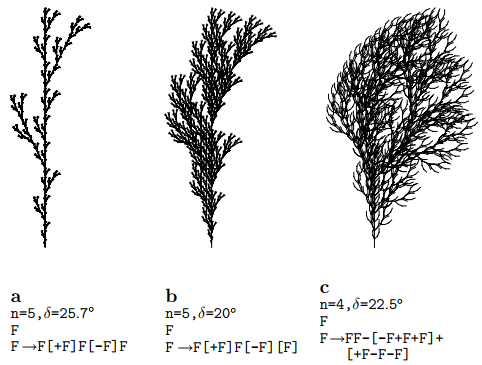
\includegraphics[width=0.5\linewidth]{obrazky-figures/ls-example.png}
    \caption{Príklad generovania stromov pomocou L-Systému\footnotemark}
    \label{fig:ls-trees}
\end{figure}

\footnotetext{Článok L-systém - \url{https://www.csh.rit.edu/~aidan/portfolio/3DLSystems.shtml}}

\subsection{Generatívna Gramatika}

Generatívne gramatiky sa používajú na opis množiny jazykových výrazov. Pomocou slov ako koncových symbolov sa prostredníctvom konečného výberu zo zoznamu rekurzívnych transformačných (alebo produkčných) pravidiel, vytvárajú nové frázy ako definuje Linden, R. a kol. vo svojej práci o procedurálnom generovaní dungeonov \cite{van2013procedural}. V PCG môžu takéto gramatiky slúžiť na generovanie rozmiestnenia miestností a smer chodieb ktoré tvoria dungeon (viď obr. \ref{fig:ls-dungeon}).

\begin{figure}[H]
    \centering
    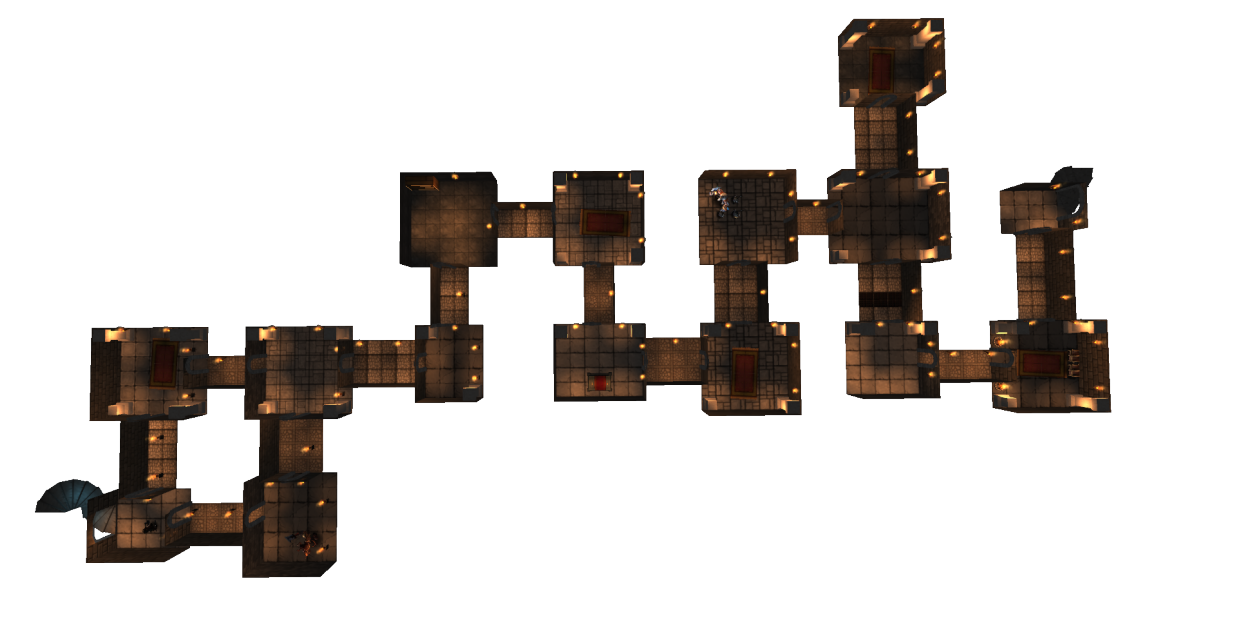
\includegraphics[width=0.4\linewidth]{obrazky-figures/gg-example.png}
    \caption{Dungeonu podľa rozloženia získaného generatívnou gramatikou \cite{van2013procedural}}
    \label{fig:ls-dungeon}
\end{figure}

\section{Jednoduché umiestňovanie miestností}

Jednoduché umiestňovanie miestností (z angl. Simple Room Placement, ďalej len SRP), táto metóda vo vopred určenej oblasti náhodne vygeneruje miestnosti a následne ich prepojí chodbami (viď obr. \ref{fig:srp}). SRP sa často používa na vytvorenie jedinečných rozložení mapy v hrách typu roguelike alebo dungeon-crawling\footnote{Článok jednoduché PCG dungeonov - \url{https://bit.ly/4a2mO9m}}.
Veľkosť a tvar jednotlivých miestnosti sa môže generovať náhodne, alebo sa vyberie miestnosť so zoznamu predom definovaných možností, pričom sa dbá aby sa navzájom neprekrývali. Posledným krokom je spájanie miestností chodbami tak, aby boli všetky miestnosti navštíviteľné hráčom. Výhoda SRP je jej jednoduchosť a možnosť pridávania komplexných pravidiel pre získanie požadovaného výsledku. 

\begin{figure}[H]
    \centering
    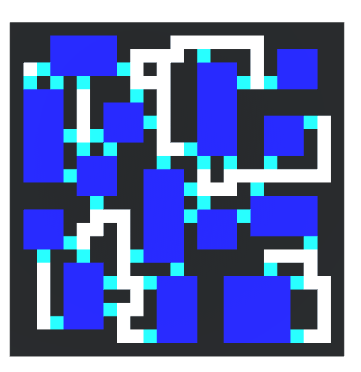
\includegraphics[width=0.3\linewidth]{obrazky-figures/srp-example.png}
    \caption{Príklad výsledku SRP s DFS prehľadávaním pre vytvorenie korirorov\footnotemark[13] }
    \label{fig:srp}
\end{figure}

Táto metóda môže poskytnúť rôznorodé výsledky podľa toho ako veľmi ju rozšírime. Nástrojmi pre ovplyvnenie výslednej mapy je spôsob výberu/generovania pôdorysu miestností a zmena algoritmu ktorým tvoríme prepájacie chodby.

\section{Náhodný krok} \label{random-walk}

Metóda náhodného kroku (z angl. Random Walk, ďalej len RW) je náhodný proces v matematickom priestore. Podľa práce Xia, F. a kol. môžeme RW definovať ako bežec, ktorý opisuje cestu pozostávajúcu z postupnosti náhodných krokov v matematickom priestore. Princíp jej fungovania je vypustenie agenta z predom daného štartovacieho bodu, a smer jeho pohybu je volený každú iteráciu behu náhodne (viď obr. \ref{fig:rw}) \cite{liangtian2020randomwalks}. 
Samotná metóda nám tak ponúka hneď niekoľko faktorov na kontrolu výsledku. Vieme meniť celkový počet krokov, počet iterácií (dĺžku behu), dĺžku jednotlivých krokov. Rozšírením týchto možností je napríklad povolenie navštívenia políčka na ktorom sme boli predchádzajúci krok (vracanie sa, angl. walk-back) alebo možnosti nastavenia pozície v novej iterácii (nový beh začne z prvotného bodu, pokračujeme z posledného bodu alebo vyberieme náhodné miesto z už prejdenej cesty).  

RW sa v PCG dá využiť na generovanie riek, ciest ale aj prirodzene vyzerajúcich jaskýň. Techniku je možné použiť aj bez ďalších algoritmov, v takom prípade musíme vygenerovať koridory pred miestnosťami (angl. corridor-first) aby sme zaručili priechodnosť mapou. Obmenou tejto metódy je takzvaná prechádzka opilcov (angl. Drunkard's Walk). V tomto prípade sa každú iteráciu náhodne vyberá miesto nového kroku, bežne sa jedná o metódu s vysokým počtom krokov alebo iterácií, takáto mapa je vhodná na hernú krajinu alebo jaskyňu.

\begin{figure}[H]
    \centering
    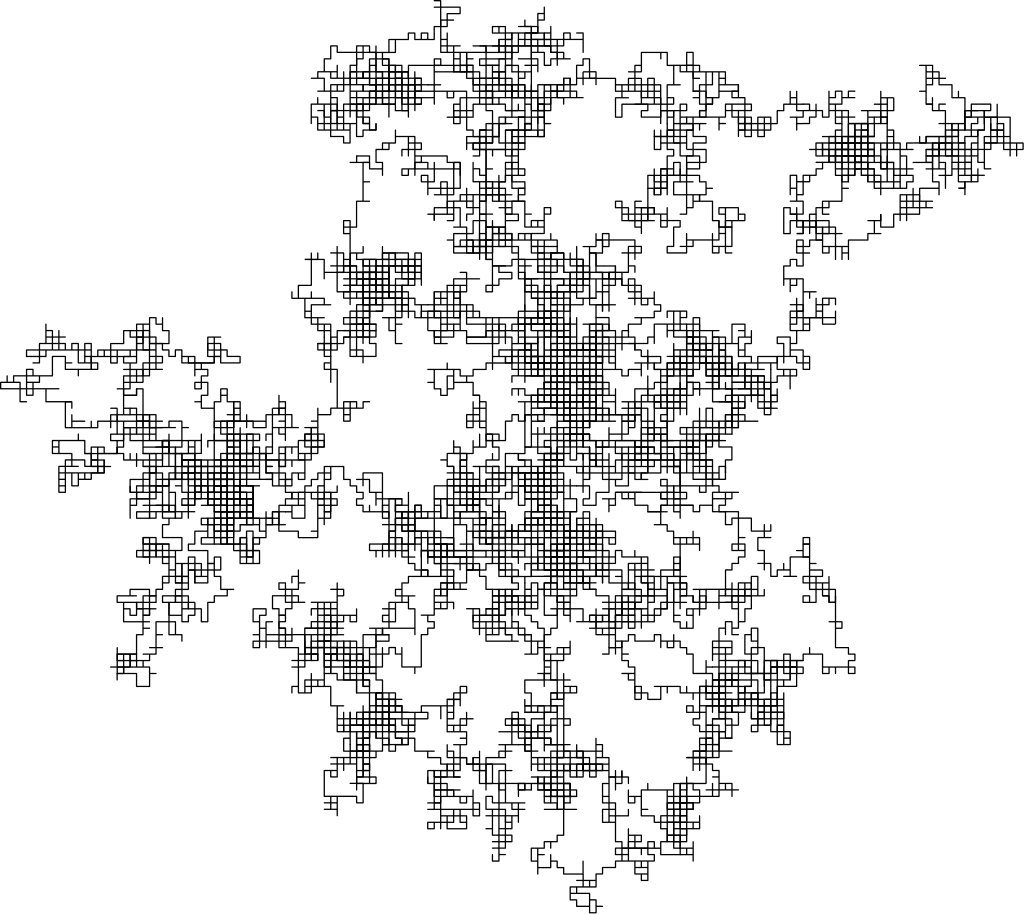
\includegraphics[width=0.35\linewidth]{obrazky-figures/dw-example.png}
    \caption{Príklad výstupu metódy náhodného kroku v 2D priestore}
    \label{fig:rw}
\end{figure}

\section{Kolaps vlnovej funkcie}

Kolaps vlnovej funkcie (z angl. Wave Function Collapse, ďalej len WFC) je algoritmus vytvárajúci dlaždicové alebo bitové mapy. Princíp jeho fungovania spočíva na rozdelení vstupného pixelového obrázka alebo úrovne založenej na dlaždiciach na malé časti a preskupuje ich z prekrývajúcich sa alebo neprekrývajúcich sa častí \cite{kim2019wfc}. Vstupný obrázok môže byť nahradený predom pevne nastavenými pravidlami. Metóda teda generuje stav buniek v novej mape zo súboru možností na základe susediacich pravidiel alebo obmedzení. Táto metóda je obzvlášť užitočná na vytváranie rôznorodých, ale súvislých vzorov a možno ju použiť pri návrhu herných úrovní a generovaní vzorov.

V PCG nachádza uplatnenie pri generovaní 2D dlaždicových máp krajín alebo dungeonov. Dá sa využiť na generovanie rozloženia predom vytvorených miestností a koridorov, generovanie rôznorodej krajiny s viacerými biommi no môže byť využitá aj na rozmiestnenie nábytku v miestnostiach. Na kontrolu metódy máme možnosť meniť samotné dlaždice a pravidlá priľahlosti alebo vstupný vzor.

\begin{figure}[H]
    \centering
    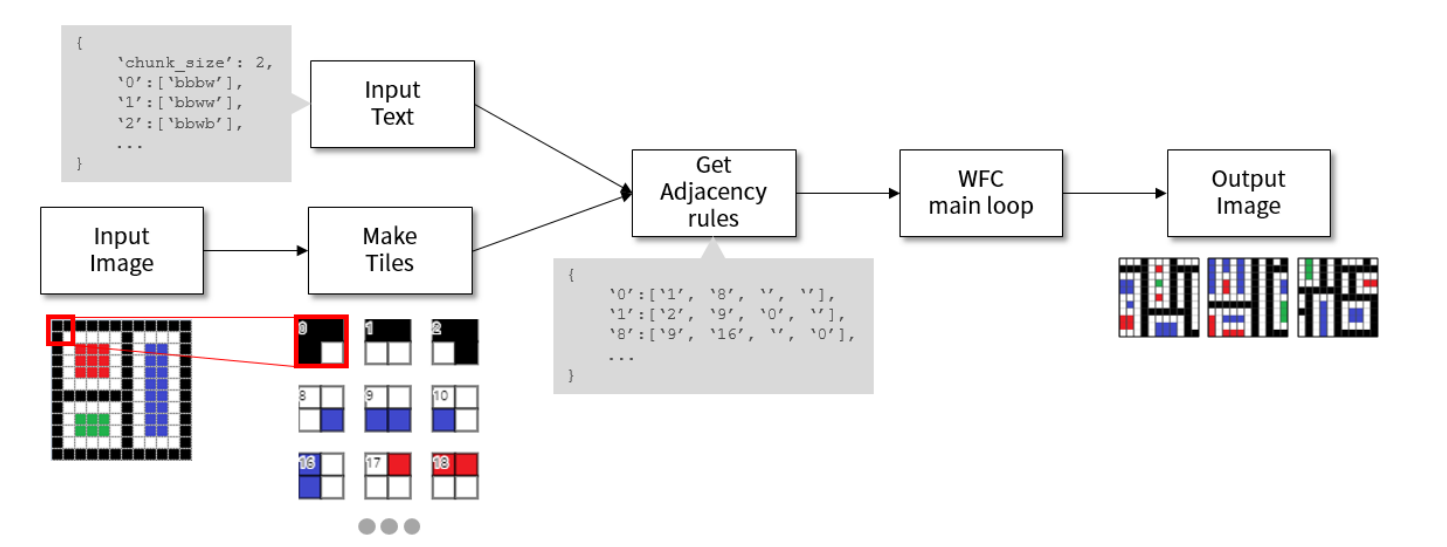
\includegraphics[width=1\linewidth]{obrazky-figures/wfc-example.png}
    \caption{Prehľad fungovania WFC metódy \cite{kim2019wfc}}
    \label{fig:enter-label}
\end{figure}

\section{Perlinov Šum}

Perlinov šum (z angl. Perlin Noise, ďalej len PN) je v kategórií šumových metód. Avšak na rozdiel od náhodného šumu, ktorý je často vizuálne nepríjemný, vytvára hladšie sa meniacu funkciu šumu \cite{kelly2006perlin}. Perlinov šum získame funkciou na počiatočné poskytnutie rozsahu hodnôt, ktoré sa následne interpolujú do koherentného šumu. Ďalším krokom sa pomocou rôznych pomerov zloží viacero vrstiev takýchto šumov, aby sa vytvorili textúru, ktorá vyzerá prirodzene a má detaily podobné fraktálom \cite{archer2011procedurally}.

V PCG sa šumy najčastejšie používajú na tvorbu textúr alebo výškových máp, ktoré sa dajú využiť na generovanie terénu (viď obr. \ref{fig:perlin-noise}). Metóda nám ponúka niekoľko parametrov na kontrolu výsledku ako frekvenciu, amplitúdu a oktávy. Frekvencia určuje rozsah, v~ktorom sa objavujú vzory šumov. Vyššia frekvencia vedie k rýchlejším zmenám vo vzore, čím sa vytvára jemnejšia a detailnejšia štruktúra. Amplitúda ovplyvňuje intenzitu zmien šumu, čo vedie k výraznejším prvkom ako sú hory. Nakoniec oktávy predstavujú vrstvenie viacerých šumov s rôznymi parametrami frekvencie a amplitúdy, každá pridaná oktáva prispeje k detailom v inej mierke, čím zvyšuje komplexnosť konečného výsledku.

\begin{figure}[H]
    \centering
    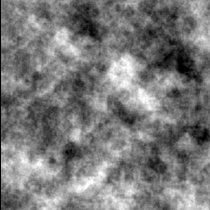
\includegraphics[width=0.3\linewidth]{obrazky-figures/perlin-noise.jpg}
    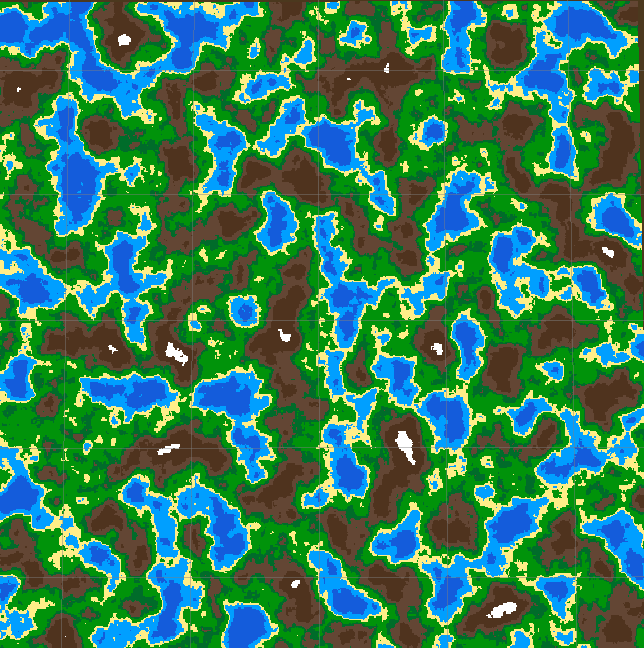
\includegraphics[width=0.3\linewidth]{obrazky-figures/perlin-map.png}
    \caption{Ukážka generovania prostredia Perlinovým šumom\protect\footnotemark}
    \label{fig:perlin-noise}
\end{figure}

\footnotetext{Projekt PCG 2D terénu - \url{https://github.com/HiGal/2D_terrain_generation}}

\section{Voronoi Diagram}

Voronoi Diagram (ďalej len VD) vieme podľa práce Aurenhammer, F. a Klein, R. definovať ako priestor rozdelený na oblasti na základe vzdialenosti k množine vopred definovaných bodov. Ku každému bodu je priradená oblasť, ktorá zahŕňa všetky miesta, ktoré sú k nemu bližšie ako k akémukoľvek inému bodu. Podľa definície je každá oblasť diagramu priesečníkom \(n-1\) otvorených pol rovín obsahujúcich miesto \(p\). Rôzne oblasti sú navzájom disjunktné \cite{aurenhammer2000voronoi}.
Na ovplyvnenie výsledku tejto metódy môžeme zmeniť počet počiatočných bodov, ich počiatočné rozmiestnenie a metódu akou sa dopočítava vzdialenosť k bodu. Metóda používa dva spôsoby výpočtu vzdialenosti medzi bodmi a to buď Euklidskú vzdialenosť (viď vzorec \ref{eq:euclid-distance}) alebo Manhattanskú (viď vzorec \ref{eq:manhattan-distance}). Samotný princíp algoritmu, je rast jednotlivých počiatočných bodov v 2D rovine každým smerom kým nenarazia na už obsadené miesto mriežky alebo hranice mapy (viď obr. \ref{fig:vd}). Tento princíp 

\begin{equation} \label{eq:euclid-distance}
\ell_{2} = d\left[\left(a_{1}, a_{2}\right), \left(b_{1}, b_{2}\right)\right] = \sqrt{(a_{1} - b_{1})^{2} + (a_{2} - b_{2})^{2}}
\end{equation}

\begin{equation} \label{eq:manhattan-distance}
d\left[\left(a_{1}, a_{2}\right), \left(b_{1}, b_{2}\right)\right] = \left| a_{1} - b_{1} \right| + \left| a_{2} - b_{2} \right|
\end{equation}

VD ako metóda je veľmi nepredvídateľná a chýba jej konzistencia výsledkov, počiatočné body sú často husté v jednej časti mapy a takmer žiadne v inej. Túto konzistenciu zlepšuje nadstavba Worleyho šumu ako Worley, S. ukazuje vo svojej práci \cite{worley1996cellular}. Samotný VD nachádza uplatnenie v PCG na generovanie hraníc biomov alebo politického, či frakčného rozdelenia na predom vytvorenej mape. Nás bude zaujímať využitie hraníc medzi jednotlivými oblasťami ako koridory pre našu mapu. Ďalšou možnosťou bude výber náhodných, nesusediacich oblastí ako miestnosti, ktoré následne prepojíme koridormi.

\begin{figure}[H]
    \centering
    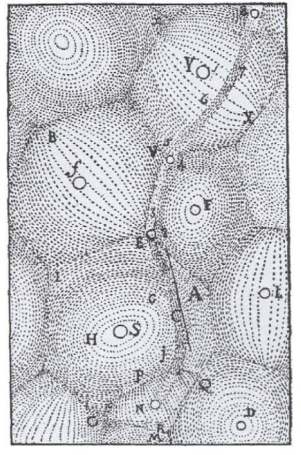
\includegraphics[width=0.22\linewidth]{obrazky-figures/vd-example.png}
    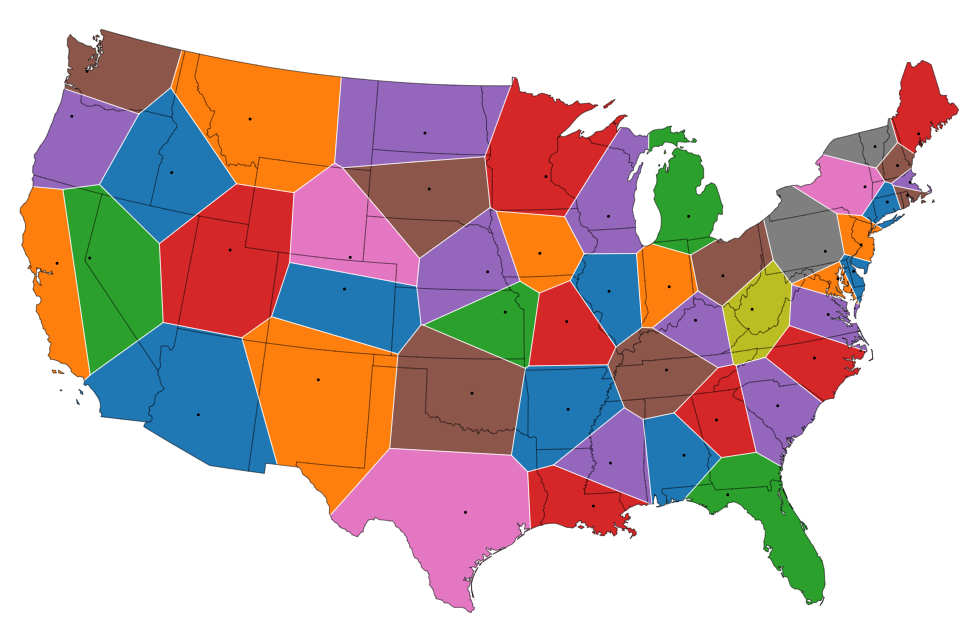
\includegraphics[width=0.55\linewidth]{obrazky-figures/vd-us.png}
    \caption{Príklad VD oblastí \cite{aurenhammer2000voronoi} a využitie VD pre výpočet hraníc štátov USA\protect\footnotemark}
    \label{fig:vd}
\end{figure}

\footnotetext{Článok spojené štáty Voronoiove - \url{https://www.jasondavies.com/maps/voronoi/us-capitals/}}

\section{Pathfinding}

Práca Ross, G. a kol. o hľadaní cesty (z angl. pathfinding) v počítačových hrách popisuje túto techniku ako systém zodpovedný za pochopenie možností pohybu vo virtuálnom priestore a vyhľadať a definovať cestu pre pohyb agenta, pričom zložité systémy sú zbytočné ak sa agent nedokáže navigovať okolo súboru prekážok. A naopak ak agent chápe svoje okolie, aj jednoduché rozhodovacie štruktúry môžu vyzerať pôsobivo \cite{graham2003pathfinding}

Vďaka správnemu implementovaniu pathfindingu sa môžu agenti navigovať okolo prekážok a dynamicky reagovať na zmeny v ich okolí. Základné algoritmy pathfindingu na ktoré sa pozrieme zahŕňajú \texttt{A*}, \texttt{Jump Point Search} a vylepšenie pohybu pomocou techniky \texttt{Context Steering}.

\subsection{A*}

\texttt{A*} je heuristický vyhľadávací algoritmus používaný v teórii grafov na určenie najlacnejšej cesty medzi uzlami v grafe. Tento algoritmus kombinuje výhody heuristickej funkcie s výhodami prehľadávania v šírke, čím zvyšuje svoju efektivitu pri prehľadávaní. Heuristická funkcia odhaduje náklady na dokončenie cesty z daného uzla. \texttt{A*} využíva túto heuristiku na určenie priorít pri rozširovaní uzlov, pričom uprednostňuje tie, ktoré sa na základe heuristického ohodnotenia javia ako bližšie k cieľu. Vo svojej práci Formálnych základov pre heuristické určenie minimálnych nákladov na cestu ho popísali Hart, P. E. a kol. \cite{hart1968formal}.

Heuristika je prístup alebo technika riešenia problému, ktorá využíva praktické metódy alebo pravidlá na rýchlejšie alebo efektívnejšie nájdenie riešenia. Medzi často používané heuristiky patria napríklad Euklidovská vzdialenosť, Manhattanova vzdialenosť\footnote{Článok A* - \url{https://theory.stanford.edu/~amitp/GameProgramming/}}.

\begin{definition}\label{def:astar}
    Predtým než si detailne rozoberieme proces akým A* pracuje, potrebujeme si definovať vlastnosti funkcií a premenných:
    \begin{itemize}
        \item \verb|s| - je počiatočným uzlom v grafe pri hľadaní cesty
        \item \verb|n| - je uzol v grafe, na začiatku sú všetky uzly \verb|"otvorené"|
        \item $g(n)$ - \textnormal{je funkcia vracajúca hodnotu doterajších nákladov na cestu od uzlu} \verb|s| do aktuálneho uzlu \verb|n| (g-skóre)
        \item $h(n)$ - je funkcia vracajúca hodnotu odhadovaných nákladov na cestu k cieľu z aktuálneho uzlu $n$ na základe vybranej heuristiky (h-skóre)
        \item $f(n) = g(n) + h(n)$ - je funkcia vracajúca hodnotu v uzle \verb|n| (f-skóre) \newline
        \hspace*{0.67cm} - nech bod \verb|n| s najnižším f-skóre je ďalším bodom na preskúmanie \newline
        \hspace*{0.67cm} - platí, že $f(s) = h(s)$ je hodnota neobmedzenej optimálnej cesty z uzlu \verb|s| k cieľu \newline
        \hspace*{0.67cm} - ďalej platí $f(n) = f(s)$ pre každý uzol \verb|n| na optimálnej ceste k cieľu
        \item T - je neprázdna množina cieľových uzlov a platí \verb|s| $\in T$ \newline
        \hspace*{0.67cm} - pre každý uzol \verb|n| je prvok \verb|t| $\in T$ preferovaným cieľom iba ak náklady na optimálnu cestu z \verb|n| do \verb|t| nepresiahnu náklady na akúkoľvek inú cestu do ktoréhokoľvek člena množiny T
        \item $\Gamma$ - je nástupnícky operátor, ktorý je v priebehu algoritmu aplikovaný na \verb|"otvorené"| uzly, aplikovaním na uzly ich rozšírime a označíme za \verb|"zatvorené"|
    \end{itemize}
\end{definition}

\noindent
Podľa definície \ref{def:astar} algoritmus pracuje v týchto krokoch:
\begin{enumerate}
    \item Označíme štartovný uzol \verb|s| za \verb|"otvorený"| a vypočítame jeho hodnotu $f(s)$

    \item Vyberieme otvorený uzol \verb|n|, ktorého hodnota $f$ je najmenšia. Remízy môžeme ľubovoľne vyriešiť, ale vždy v prospech niektorého z uzlov \verb|n| $\in T$
    
    \item Ak \verb|n|$ \in T$, označíme \verb|n| ako \verb|"uzavretý"| a ukončíme algoritmus
    
    \item V opačnom prípade označíme \verb|n| za \verb|"uzavretý"| a použijeme jeho následníka
    $\Gamma$ na \verb|n|. Vypočítame $f$ pre každého následníka \verb|n| a
    každého následníka, ktorý ešte nebol označený ako \verb|"uzavretý"|, označíme ako \verb|"otvorený"|.
    Za \verb|"otvorený"| označíme každý \verb|"uzavretý"| uzol \verb|n|, ktorý je nasledovníkom
    \verb|n| a pre ktorý je $f(n_i)$ teraz menšie, ako bolo v čase, keď bol $n_i$,
    označený ako \verb|"uzavretý"|. A vrátime sa na krok 2.
\end{enumerate}

\begin{figure}[H]
    \centering
    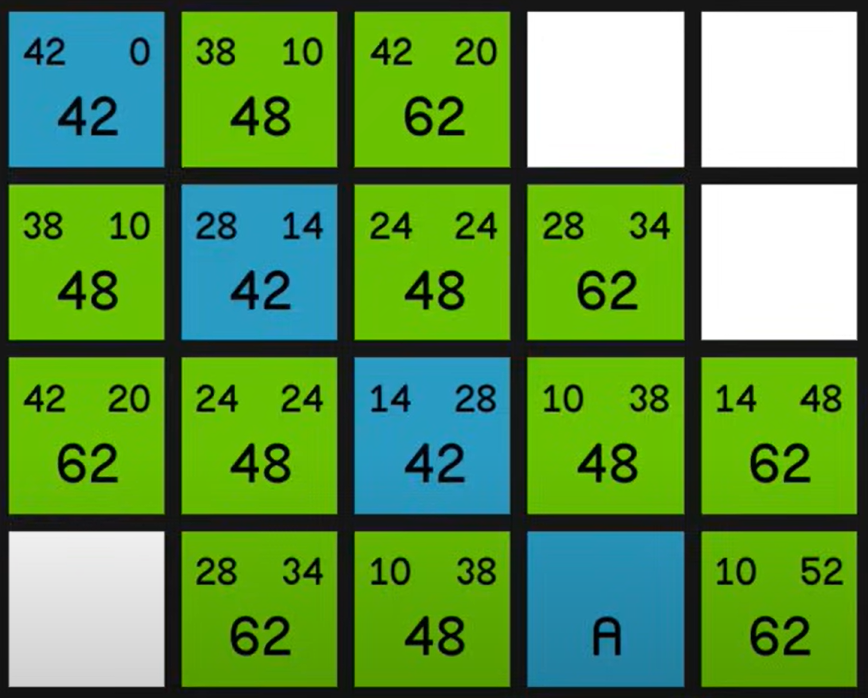
\includegraphics[width=0.35\linewidth]{obrazky-figures/astar.png}
    \includegraphics[width=0.42\linewidth]{obrazky-figures/astarľ.png}
    \caption{Ukážka procesu hľadania cesty, štartovací bod v uzle \texttt{A}, koncový bod v ľavom hornom rohu. Hodnoty uzlu: f-skóre v strede, g-skóre vľavo hore, h-skóre vpravo hore. Farba uzlov: zelená - otvorené, modrá - výsledná cesta, červená - uzavreté, čierna - prekážky\protect\footnotemark .}
    \label{fig:astar}
\end{figure}

\footnotetext{Video ukážka fungovania JPS - \url{https://www.youtube.com/watch?v=-L-WgKMFuhE}}

\subsection{Jump Point Search}

Práca Harabor, D. a Grastien, A. popisuje vyhľadávanie skokových bodov (z angl. Jump Point Search, ďalej len JPS) ako algoritmus na hľadanie ciest špeciálne navrhnutý pre prostredia s 2D mriežkou. Vylepšuje tradičné metódy vyhľadávania \texttt{A*} (viď obr. \ref{fig:astar_vs_jps}). A to strategickým výberom bodov v  mriežke (body skoku) na ďalšie preskúmanie. Tieto skokové body sa vyberajú na efektívnu navigáciu v prostredí a nájdenie cesty medzi štartovacou a cieľovou pozíciou \cite{harabor2011online}.

\noindent
Ďalej podľa tejto práce algoritmus pracuje v týchto krokoch:
\begin{enumerate}
    \item Počiatočný uzol pridáme do otvorenej množiny. Inicializujme náklady a ukazatele na rodičov pre každý uzol.

    \item Z otvorenej množiny vyberieme uzol s najnižšou cenou. Pre každého nasledovníka tohto uzla použijeme JPS na určenie, či pozdĺž smeru pohybu existujú nejaké skokové body. Ak sa nájde bod skoku, pridáme ho do otvorenej množiny.

    \item Bod skoku je nasledujúci uzol, ktorý poskytuje výrazné zlepšenie dĺžky cesty v porovnaní so svojím predchodcom. Body skoku sa identifikujú rekurzívnym pohľadom dopredu pozdĺž každého smeru pohybu, kým sa nenarazí na prekážku alebo sa nenájde bod skoku.

    \item Vyčistíme nepotrebné uzly z prehľadávaného priestoru vynechaním určitých uzlov, ktoré neprispievajú k nájdeniu optimálnej cesty. Tento proces orezávania zníži počet uzlov, ktoré je ešte potrebné preskúmať.

    \item Pokračujeme v rozširovaní uzlov a identifikácii bodov skoku, kým nedosiahneme cieľový uzol alebo kým už nie sú žiadne ďalšie uzly na preskúmanie.

    \item Po dosiahnutí cieľového uzla zrekonštruujeme cestu spätným sledovaním nadradených ukazovateľov z cieľového uzla do počiatočného uzla.
\end{enumerate}

\begin{figure}[H]
    \centering
    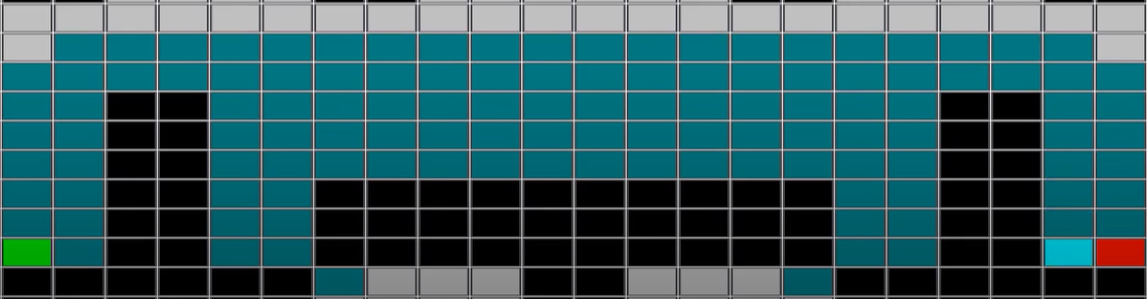
\includegraphics[width=0.60\linewidth]{obrazky-figures/astar3.png}
    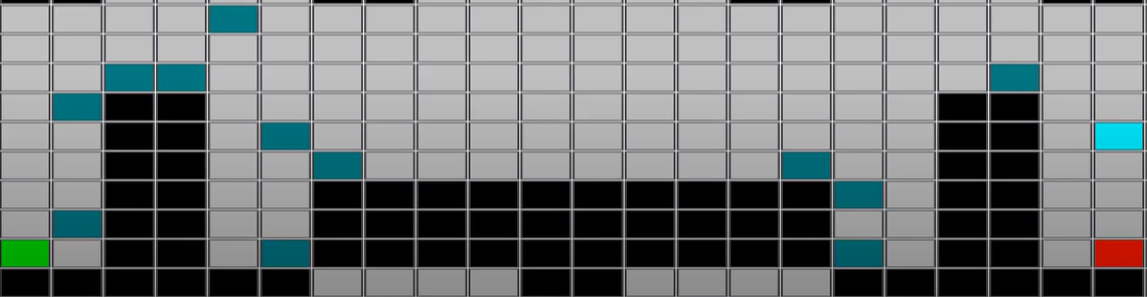
\includegraphics[width=0.60\linewidth]{obrazky-figures/jps.png}
    \caption{Vizuálne porovnanie počtu prehľadaných (tmavomodrých) uzlov algoritmami A* (hore) a JPS (dole)\protect\footnotemark }
    \label{fig:astar_vs_jps}
\end{figure}

\footnotetext{Porovnanie A* a JPS - \url{https://www.youtube.com/watch?v=ROG4Ud08lLY}}

\subsection{Context Steering}

Kontextové riadenie (z angl. context steering, ďalej len CS) resp. riadenie poháňané správaním (z angl. behavior-driven steering) je v hernom priemysle technika ktorá dovoľuje agentovi pri pohybe reagovať na svoje okolie dynamicky a to aj v nasledovania cesty k cieľu. Nezameriavame sa pri tom na hľadanie najkratšej cesty, ale zohľadňujeme rôzne faktory ako typ terénu a dynamické aj statické prekážky. Táto technika nachádza využitie v robotike, umelej inteligencii aj modeloch správania živočíchov. V hernom priemysle sa využíva pri modeloch vozidiel v 2D aj 3D. Agenti sa vďaka tomu môžu pohybovať v priestore inteligentnejšie a zohľadniť pri pohybe aktuálny stav hry \cite{reynolds1999steering}.

Práca Fray, A. popisuje fungovanie CS pomocou kontextových máp, ktoré predstavujú záujmy subjektu v rámci prostredia. Tieto mapy premietajú faktory prostredia do kruhového poľa, pričom každý povolený smer pohybu má vlastnú hodnotu a jeho príslušná intenzita predstavuje preferenciu alebo averziu správania. Pre náš problém využijeme dve kontextové mapy s ôsmimi smermi pohybu. Odčítaním týchto máp dospejeme ku konečnému rozhodnutiu (viď obr. \ref{fig:cs}), ktoré je v súlade s celkovými cieľmi agenta a zároveň zohľadňuje kontextové vplyvy \cite{fray2019context}.

Z výslednej mapy vyberieme smer s najvyššou hodnotou a aplikujeme ho na agentov pohyb. Výsledok však môže byť zubatý, v zmysle rýchlych zmien v smere, preto vypočítame priemerný vektor pohybu, ktorý normalizujeme a vytvoríme tak plynulý pohyb.

\begin{figure}[H]
    \centering
    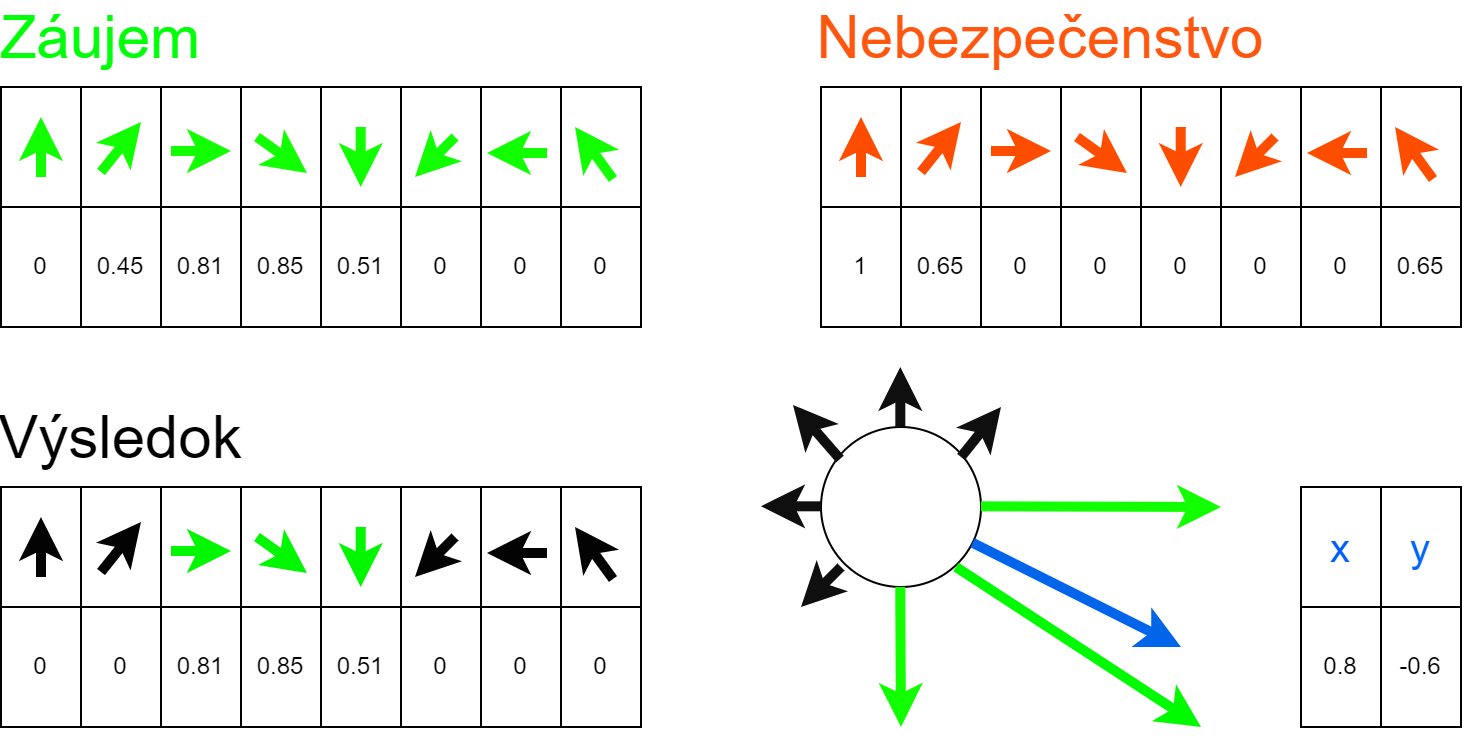
\includegraphics[width=0.9\linewidth]{obrazky-figures/cs.png}
    \caption{Princíp získania smeru technikou kontextového riadenia, odčítaním smeru prekážok (nebezpečenstvo) od smerov záujmu agenta a následná normalizácia priemeru výsledných smerov}
    \label{fig:cs}
\end{figure}

\chapter{Návrh hry}

V tejto kapitole stručne predstavíme proces navrhovania hier so zameraním na koncept minimálneho životaschopného produktu (z angl. Minimal Viable Produt, ďalej len MVP). Tento prístup využívame pretože vývoj hier je komplexný a časovo náročný proces, ktorý zahŕňa naratívne aj audiovizuálne prvky. Tieto prvky však nie sú primárnym cieľom tejto práce.

Ako spomína práca Aleema, S. a kol. existujú tri hlavné fázy, ktoré tvoria proces vývoja hry \cite{aleem2016game}. Medzi tieto fázy patrí pred produkcia, produkcia a postprodukcia. V rámci tejto kapitoly sa zameriame najmä na pred produkčnú fázu. Stanovíme si špecifiká hry, poskytneme stručný prehľad herného systému, zvolíme si grafický štýl a začneme vyvíjať prototyp. Týmto zjednodušeným postupom sa vyhneme podrobnému návrhu, ktorý by mal zahŕňať aj audiovizuálnu a príbehovú časť hry.

\section{Špecifikácia Požiadaviek}

Zvolili sme si akčný, roguelike žáner a to z dôvodu aby sme ukázali prínos generovania máp. Pre hry tohoto žánru je dôležitá znovu hrateľnosť a generovaním vieme hráčom ponúknuť unikátne mapy pri každom spustení. Zároveň je dôležité aby sa generovanie máp nestalo hlavnou mechanikou hry. Účelom použitia PCG v tejto práci je ukázať, ako sa dajú použiť rôzne metódy na vytvorenie zaujímavých a rozmanitých prostredí pre hru ktorá by fungovala a bola zábavná aj so statickou mapou ako napríklad hry Vampire Survivors a Brotato.

Ďalšou dôležitou súčasťou nášho návrhu je rozhodnutie vytvoriť hru v 2D s pohľadom zhora. Toto rozhodnutie zohráva kľúčovú úlohu pri zjednodušení celkovej štruktúry hry, ako aj úrovne zložitosti procesu procedurálneho generovania.

Hra bude mať pixelovú grafiku s veľkosťou spritu $16\times16$ pixelov s preddefinovanou vhodnou paletou farieb. Aby sme hru zaobalili do jednoduchého príbehu, zvolíme si za hlavnú postavu ducha ktorý vie posadnúť telá nepriateľov alebo robotov, ovládať ich. Krotého cieľom je poraziť zlého čarodeja na konci dungeonu.

\section{Herný systém}

V rámci roguelike žánru sa budeme držať osvedčených konvencií a pravidiel, ktoré definuje Harris, J. vo svojej práci v kapitole Osem pravidiel roguelike dizajnu \cite{harris2020exploring}.

Niektoré z týchto pravidiel však porušíme. Naša hra nebude ťahová a inšpirovať sa bude titulmi ako Darkest Dungeon či Wizard of Legend. Vytvoríme statickú mapu mesta, kde si hráč bude môcť vylepšovať svoje schopnosti a následne sa vydávať na výpravy do procedurálne generovaných dungeonov. V základnej verzii hry bude mať po každej úrovni dungeonu možnosť vrátiť sa do mesta a nakúpiť si vylepšenia.

Náročnosť hry bude exponenciálne rásť, čím sa stane zdanlivo neprekonateľnou a~prinúti hráča využiť všetky svoje znalosti a mechaniky hry. Podmienkou pre návrat do mesta po každej úrovni bude súboj s bossom alebo elitnou jednotkou.

\subsection{Postavy}

V hre sa hráč stretne s tromi frakciami postáv, s ktorými bude môcť interagovať:

\begin{enumerate}
    \item Strážcovia
    \begin{itemize}
        \item Priateľská frakcia, ktorá ponúkne hráčovi pomoc a vylepšenia v meste.
        \item Budú slúžiť ako sprievodcovia a poradcovia, čím uľahčia hráčovi napredovanie.
        \item Ponúknu rôzne služby a tovary, ktoré posilnia hráčove šance na prežitie.
    \end{itemize}

    \item Okultisti
    \begin{itemize}
        \item Nepriateľská frakcia, ktorú bude musieť hráč poraziť v boji.
        \item Budú predstavovať hrozbu a prekážku na hráčovej ceste.
        \item Ich porážka prinesie hráčovi cenné odmeny a posunie ho bližšie k víťazstvu.
    \end{itemize}

    \item Golemovia
    \begin{itemize}
        \item Neutrálna frakcia duchov obývajúcich telá golemov.
        \item Ponúknu hráčovi svoje stroje a vylepšenia výmenou za splnenie určitých úloh.
    \end{itemize}
\end{enumerate}

\subsection{Herný cyklus a mechaniky}

Hra ponúkne vyvážený herný zážitok, ktorý kombinuje oddych a vylepšovanie v meste s~akčným bojom v dungeone (viď obr. \ref{fig:cycle}). V meste si hráč môže oddýchnuť, vylepšiť svoje vybavenie a schopnosti a pripraviť sa na ďalšie výzvy. V dungeone bude čeliť presile nepriateľov, aby získal suroviny na vylepšenie a zvýšil si tak šancu poraziť ťažších nepriateľov a~bossov.

Hráč sa bude pohybovať pomocou kláves \verb|WASD|, mierenie kurzorom a útoky pomocou tlačidiel myšky a medzerníku. Ďalej bude mať možnosť prebrať kontrolu nad nepriateľmi po namierení kurzoru a stlačení medzerníku (viď obr. \ref{fig:possess}). Táto mechanika bude fungovať pomocou raycastingu, aby sa zabránilo prenikaniu cez steny. Z posadnutého nepriateľa sa dostane späť do formy ducha opätovným stlačením medzerníku. Interakcie s prostredím a~postavami bude zahájená po stlačení \verb|E| na klávesnici.

\begin{figure}[H]
    \centering
    
\includegraphics[width=1\linewidth]{obrazky-figures/cycle.png}
    \caption{Vizualizácia základného herného cyklu medzi scénami a hráčove aktivity}
    \label{fig:cycle}
\end{figure}

\begin{figure}
    \centering
    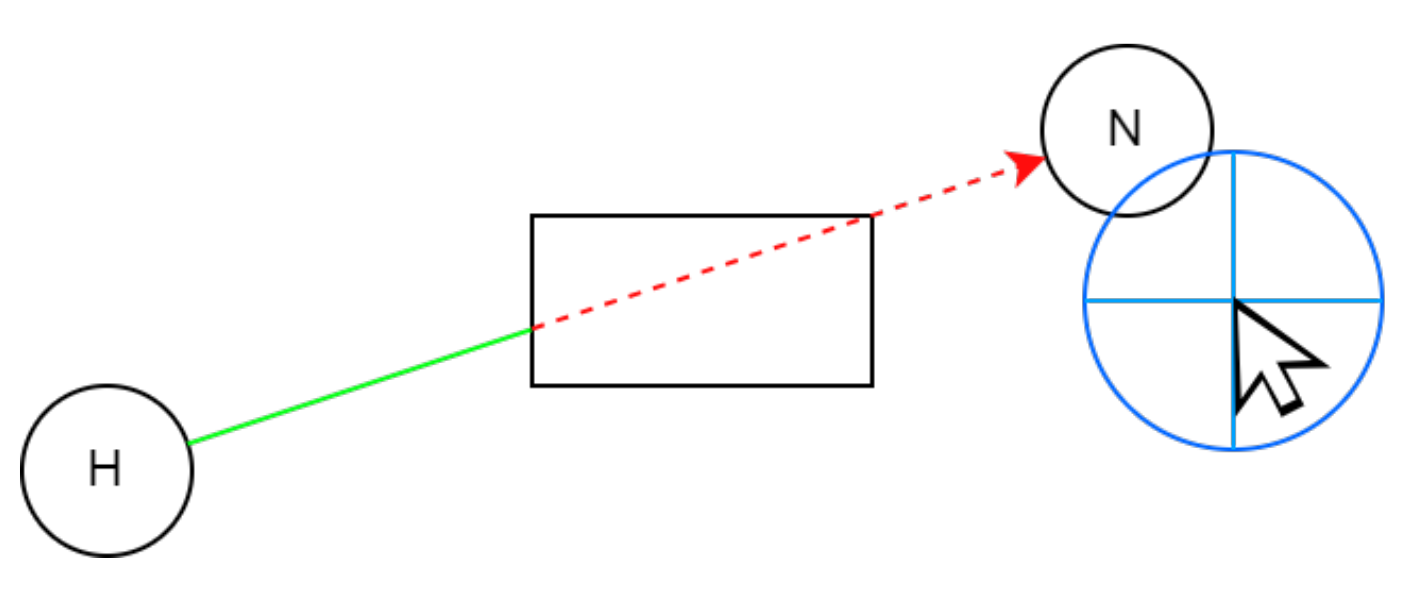
\includegraphics[width=0.5\linewidth]{obrazky-figures/possess.png}
    \caption{Mechanika posadnutia, pre posadnutie musí raycasting od hráča (H) bez prerušenia prekážkou dopadnúť na náhodne vybraného nepriateľa (N) v blízkom okolí kurzoru}
    \label{fig:possess}
\end{figure}

\subsection{Schopnosti}

Hráč ako duch nemá žiadne schopnosti, tie získa v závislosti od typu tela, ktoré obýva. Väčšina útokov bude pozostávať z projektilov rôznych veľkostí a efektov. Hráč môže priamo vylepšovať iba golema, ktorý sa prenáša medzi mapami a automaticky sa opravuje. Vylepšenia rozdelíme na 2 typy:

\begin{itemize}
    \item Pasívne efekty - Platia pre akékoľvek obývané telo:
    \begin{itemize}
        \item Zväčšenie projektilu a jeho útoku
        \item Zrýchlenie projektilu a jeho čas na zvonu použitie (angl. cooldown)
        \item Odomknutie špeciálnych efektov pre jednotlivé schopnosti
    \end{itemize}
    \item Vylepšenia golema:
    \begin{itemize}
        \item Výmena schopností
        \item Zvýšenie života
        \item Zvýšenie rýchlosti pohybu
    \end{itemize}
\end{itemize}

\subsection{Nepriatelia}

Plánujeme zakomponovať 3 typy nepriateľov:

\begin{enumerate}
    \item Agilný nepriatelia na blízko
    \begin{itemize}
        \item Náhodne sa pohybujú po mape a hľadajú hráča.
        \item Po zistení hráča ho aktívne prenasledujú. 
    \end{itemize}
    \item Mágovia strieľajúci z diaľky
    \begin{itemize}
        \item Stacionárne jednotky s magickými útokmi na diaľku.
        \item Majú zvýšený okruh detekcie hráča.
    \end{itemize}
    \item Obrancovia s vysokým životom a útokom
    \begin{itemize}
        \item Silný no pomalý nepriatelia s vysokou odolnosťou a silnými útokmi.
        \item Hliadkujú na predom vygenerovanej ceste okolo dôležitých bodov.
    \end{itemize}
    \item Elitné verzie predošlých typov ktoré sa nedajú ovládať
    \begin{itemize}
        \item Silnejšie a odolnejšie verzie bežných nepriateľov.
        \item Nedajú sa ovládať hráčom.
        \item Vdýchnu hre väčšiu výzvu a variabilitu.
    \end{itemize}
    \item Bossovia, podobne ako elítne jednotky budú neposadnuteľné a budú mať odlišné útoky
    \begin{itemize}
        \item Najsilnejší typ nepriateľa v hre.
        \item Majú unikátne útoky a mechaniky.
        \item Na základe počtu živých nepriateľov na mape dostanú bonus k životom a privolajú si pomocníkov.
    \end{itemize}
\end{enumerate}

Pre dynamické prenasledovanie hráča v teréne využijeme \verb|context steering|\footnote{Context Steering - Fray, A. \url{https://bit.ly/3WrjhOD}}. Naopak, pre efektívne a predvídateľné hliadkovanie, ktoré uľahčí orientáciu v prostredí, sa spoľahneme na hľadanie cesty použitím \verb|A*| algoritmu.

\section{Grafický štýl a UI}

Pre potreby našej hry sme sa rozhodli vytvoriť originálnu pixelovú grafiku s rozlíšením 16x16 pixelov. Toto rozlíšenie, hoci pomerne nízke, nám umožňuje zachovať prehľadnosť a zároveň dodáva hre retro vzhľad, ktorý je pre daný typ hry ideálny.

Pre každú frakciu v hre sme definovali vlastnú paletu farieb, aby sme zachovali jednotný vizuálny štýl a uľahčili hráčom rozpoznanie frakcií na bojisku. Pri tvorbe paliet sme sa inšpirovali osvedčenými princípmi teórie farieb a využili dostupné online zdroje a nástroje, ako napríklad \verb|LOSPEC|\footnote{Nástroj na výber farieb LOSPEC - \url{https://lospec.com/palette-list}}.

Spomínané rozlíšenie $16\times16$ pixelov síce prináša určité obmedzenia, no zároveň nám umožňuje udržať hru v rámci rozsahu a cieľov projektu. Vyššie rozlíšenie by bolo pre takýto projekt náročné na tvorbu a presiahlo by naše technické aj časové možnosti (viď obr. \ref{fig:chars}). Z rovnakého dôvodu sme sa zatiaľ rozhodli pre zjednodušenie animácií postáv. Animácie vytvoríme pomocou zmien rozmerov a rotácie v hernom engine.

\begin{figure}[H]
    \raggedright
    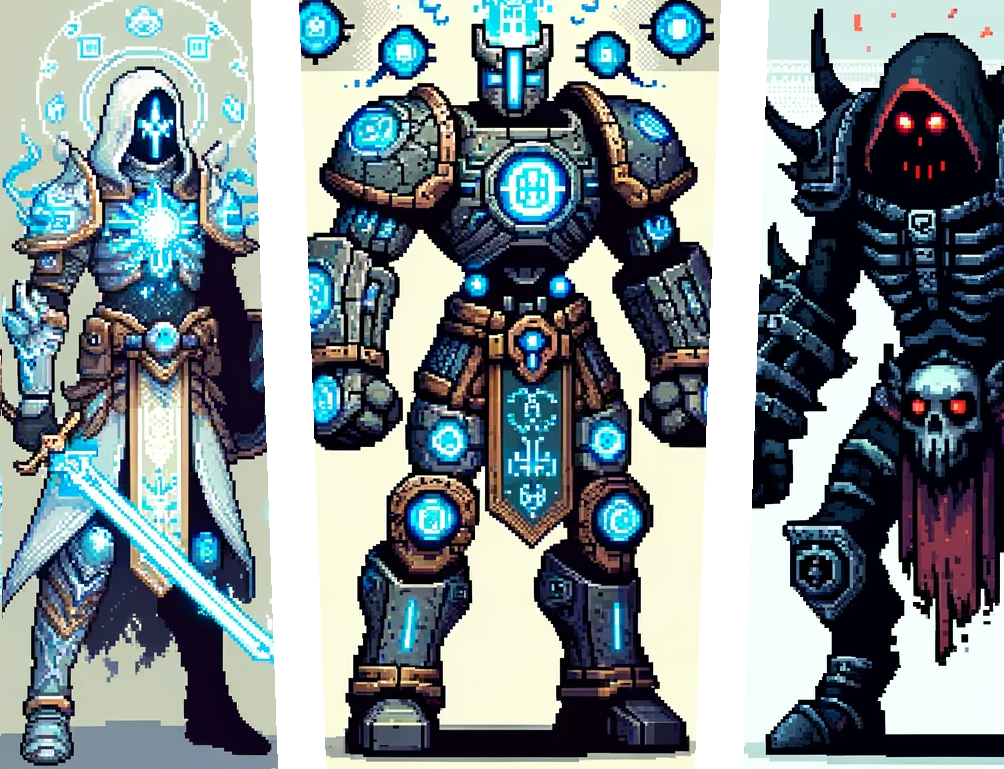
\includegraphics[width=0.45\linewidth]{obrazky-figures/chars.png}
    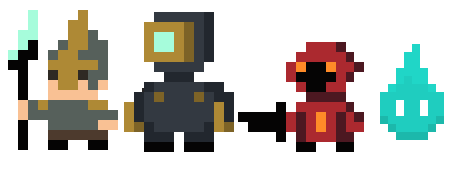
\includegraphics[width=0.5\linewidth]{obrazky-figures/chars2.png}
    \caption{Ilustračné obrázky grafiky postáv vľavo, grafika ktorú použijeme v hre vpravo}
    \label{fig:chars}
\end{figure}

Na zabezpečenie plynulého herného zážitku chceme vytvoriť jednoduché prehľadné užívateľské rozhranie (z angl. user interface, ďalej len UI). Hra v tejto práci bude mať tri samostatné obrazovky: mesto, dungeon a menu. Každá obrazovka má svoju osobitnú funkciu, a aby ju návrh UI efektívne plnil, je potrebné každú obrazovku dôkladne naplánovať. Pri spustení hry budeme rozlišovať stav, či existuje uložený záznam o hre (viď obr. \ref{fig:screen-menu-game}). Ďalej pri tvorení novej hry dáme hráčom možnosť zvoliť si parametre sveta ako obtiažnosť, veľkosť máp a typ metódy generovania mapy (viď obr. \ref{fig:screen-settings}). Na obrazovke samotnej hry bude potrebovať hráč sledovať tri základné bloky, život hráča, schopnosti a život tela v ktorom sa aktuálne nachádza (viď obr. \ref{fig:screen-menu-game}) \footnotemark.

\begin{figure}[H]
    \centering
    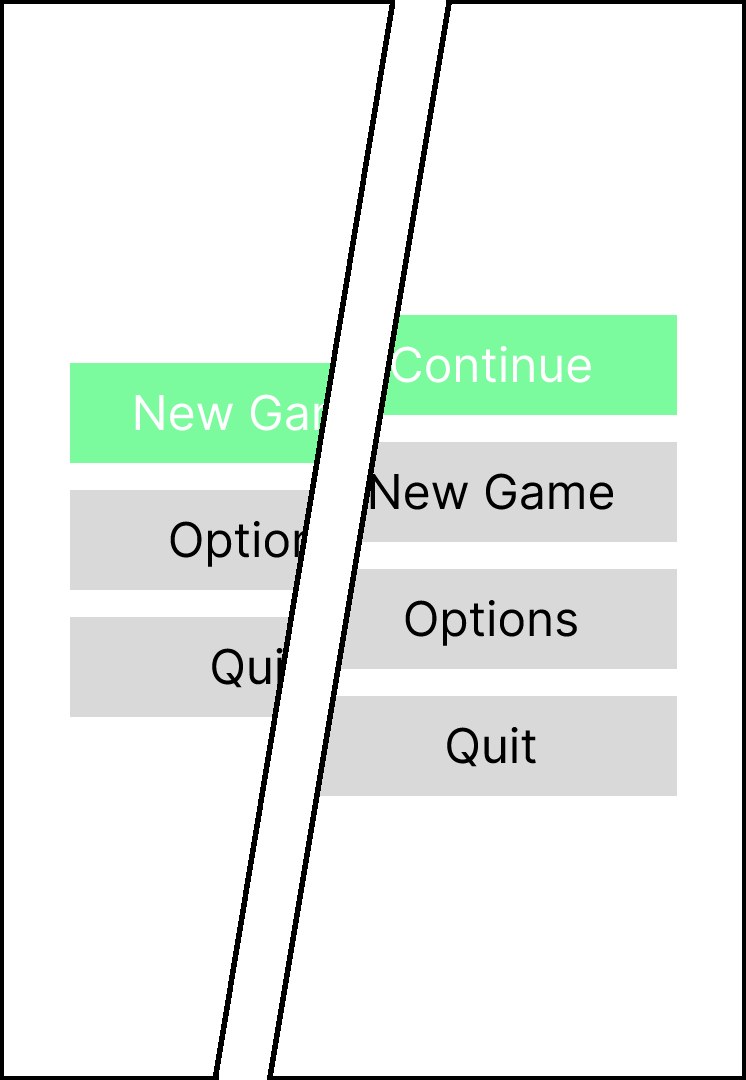
\includegraphics[width=0.30\linewidth]{obrazky-figures/screen-menu.png}
    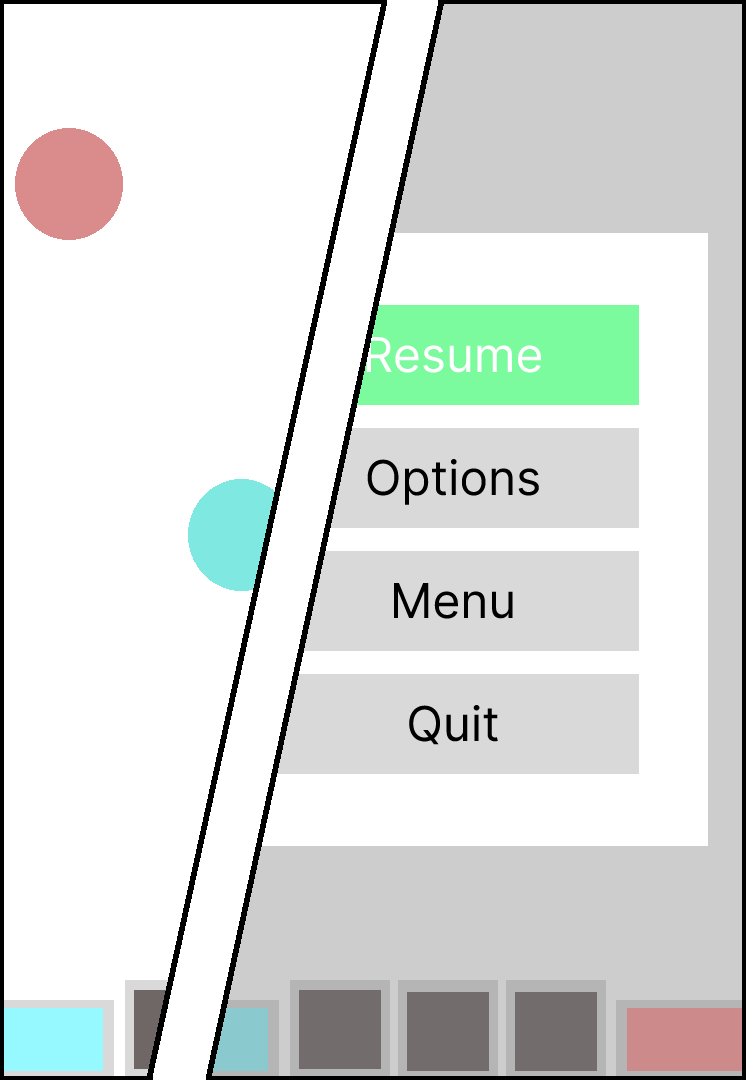
\includegraphics[width=0.30\linewidth]{obrazky-figures/screen-game.png}
    \caption{Dvojice obrázkov, vľavo - obrazovky menu meniace sa na základe, či už bola hra niekedy spustená, vpravo - obrazovky hry zobrazujúce rozloženie životov, schopností hráča a escape menu}
    \label{fig:screen-menu-game}
\end{figure}

\begin{figure}[H]
    \centering
    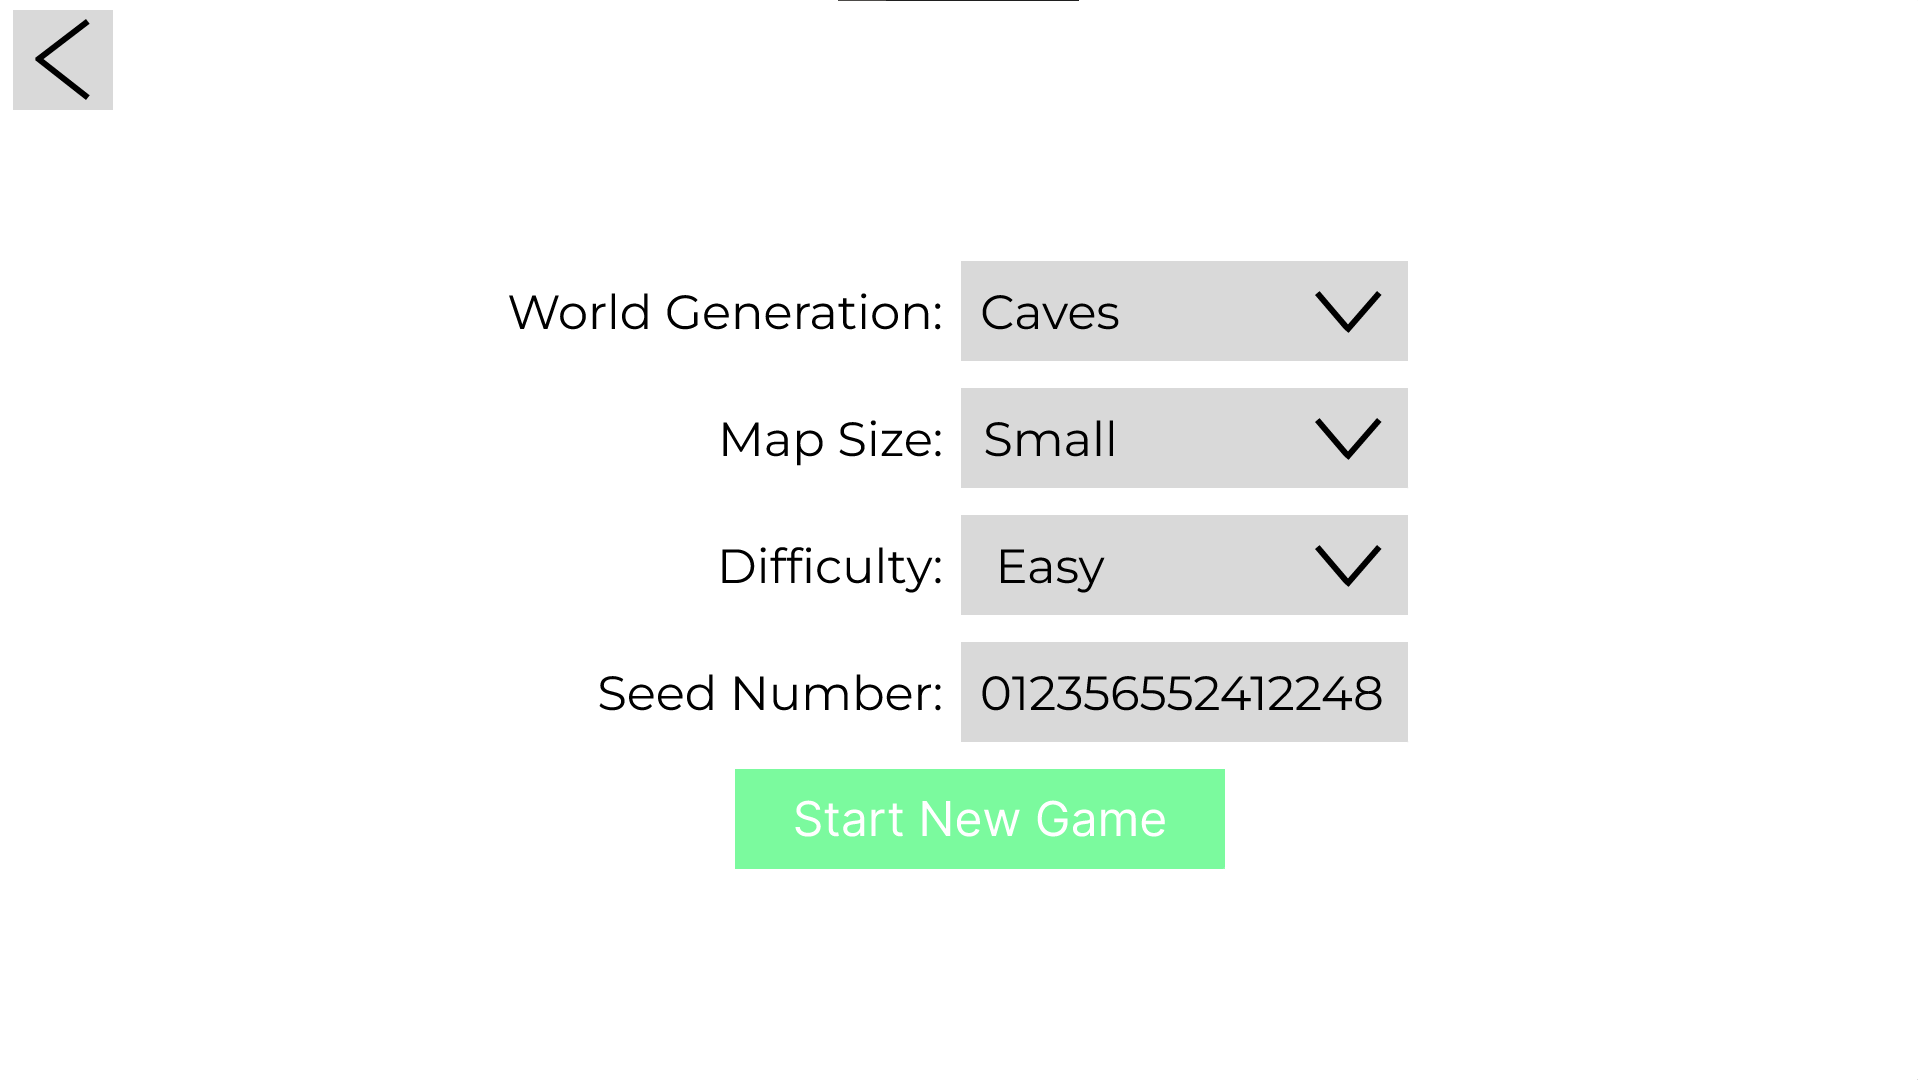
\includegraphics[width=0.8\linewidth]{obrazky-figures/screen2.png}
    \caption{Výber nastavení pri tvorbe novej hry, pod vhodnými aliasmi skryjeme názvy metódy podľa tvarov ktoré pri generovaní vytvárajú}
    \label{fig:screen-settings}
\end{figure}

\footnotetext{Celý návrh vo figme - \url{bit.ly/44z4Vhs}}

\chapter{Implementácia} \label{sec:implementation}

V tejto kapitole si detailne rozoberieme implementáciu nášho projektu. Pre naše potreby sme si zvolili herný engine Unity. Rozhodli sme sa preň pre jeho popularitu a použiteľnosť v rôznych žánroch hier. Unity je všestranný engine v ktorom vznikli mnohé akčné 2D hry, ako je Cuphead či stratégie ako Rimworld. Okrem toho dokáže efektívne spracovať aj komplexné 3D prostredia, čo plne využívajú tituly ako Subnautica a Rust. Jeho flexibilitu dokazuje aj využitie pre menšie nezávislé projekty, kde môžeme uviesť príklad Lethal Company od jediného vývojára s prezývkou Zeekerss. Ale aj vo veľkých herných produkciách, ako je kartová hra Hearthstone od Blizzard Entertainment. S Unity teda máme k dispozícii všetky potrebné nástroje na realizáciu nášho projektu. V rámci Unity enginu sme programovali v jazyku \verb|C#| s použitím \verb|.NET Framework 4.x| a \verb|.NET Standard 2.0.| Potrebné informácie sme získavali z oficiálnych dokumentácií spoločnosti Microsoft a manuálov Unity. Samotná aplikácia je vytvorená na verzii Unity \verb|2021.3.8f1|.

Súčasťou kapitoly  je prehľad scén, z ktorých je aplikácia zložená, detailný pohľad na návrh štruktúry a procesu procedurálneho generovania máp, dogenerovanie stien, implementácia mechaník a vizuálnych prvkov. 

\section{Scény}

V našej aplikácii budeme plynulo prechádzať medzi rôznymi scénami. Pre lepšie organizovanie a oddelenie jednotlivých logických častí sme ich rozdelili na \verb|Menu|, \verb|Dungeon| a \verb|City|. Pričom každá scéna spĺňa inú úlohu v celkovej architektúre hry a pre plynulé prepínanie medzi nimi sme vytvorili pomocné UI okno pre načítanie \verb|Loading|. Toto okno sa zapne vždy pri prechode medzi scénami a slúži ako vizuálna odozva aby hráč vedel, že jeho akcie boli hrou spracované.

Scény \verb|Dungeon| a \verb|City| budú zdieľať valnú väčšinu UI prvkov s rozdielom, že v meste hráč nebude v nebezpečí a bude mať čas na oddych.

\begin{figure}[H]
    \centering
    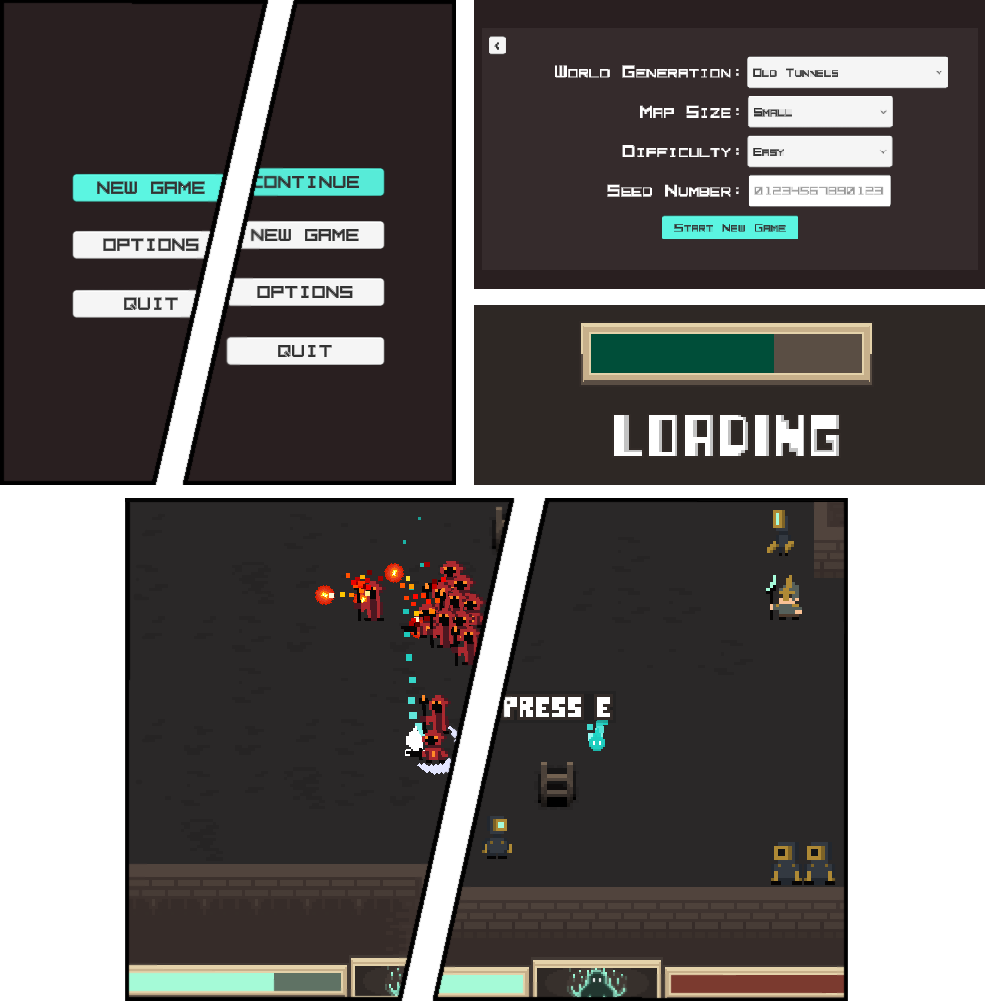
\includegraphics[width=1\linewidth]{obrazky-figures/screens.png}
    \caption{Ukážka scén Menu pri novej hre/pokračovaní, výber nastavení a UI blok načítania hore, scéna dungeonu/mesta dole}
    \label{fig:scenes}
\end{figure}

\section{Generovanie}

Celý proces generovania od zvolenia seedu až po vizualizáciu mapy je rozdelený na 6 až 7 časti v závislosti od schopností daných metód. A prebieha pri ňom komunikácia viacerých objektov a načítanie z registrov \verb|PlayerPrefs| do ktorých si pri vytváraní novej hry zapíšeme parametre generovania (viď obr. \ref{fig:scenes}). 

\begin{enumerate}
  \item Inicializácia
  \begin{enumerate}[label*=\arabic*.]
    \item Zadanie/vygenerovnie\,seedu,\,výber\,obiažnosti,\,veľkosť\,mapy,\,metóda\,generovania
    \item Načítanie nastavení, nastavenie generátoru, výber a inicializácia generátoru
  \end{enumerate}
  
  \item Generovanie
  \begin{enumerate}[label*=\arabic*.]
    \item Generovanie miestností, koridorov, plochy mapy
    \item Kontrola mapy pomocnými algoritmami na overenie prechodnosti mapy a mazanie nedostupných častí (A*, flood fill)
    \item Nastavenie štartovacieho a cieľového bodu na mape, umiestnenie nepriateľov
  \end{enumerate}
  
  \item Vizualizácia
  \begin{enumerate}[label*=\arabic*.]
    \item Generovanie grafiky stien
    \item Vizualizácia a nastavenie collider-u (nepriechodná prekážky) na 2D mriežke
  \end{enumerate}
\end{enumerate}

\begin{figure}[H]
    \centering
    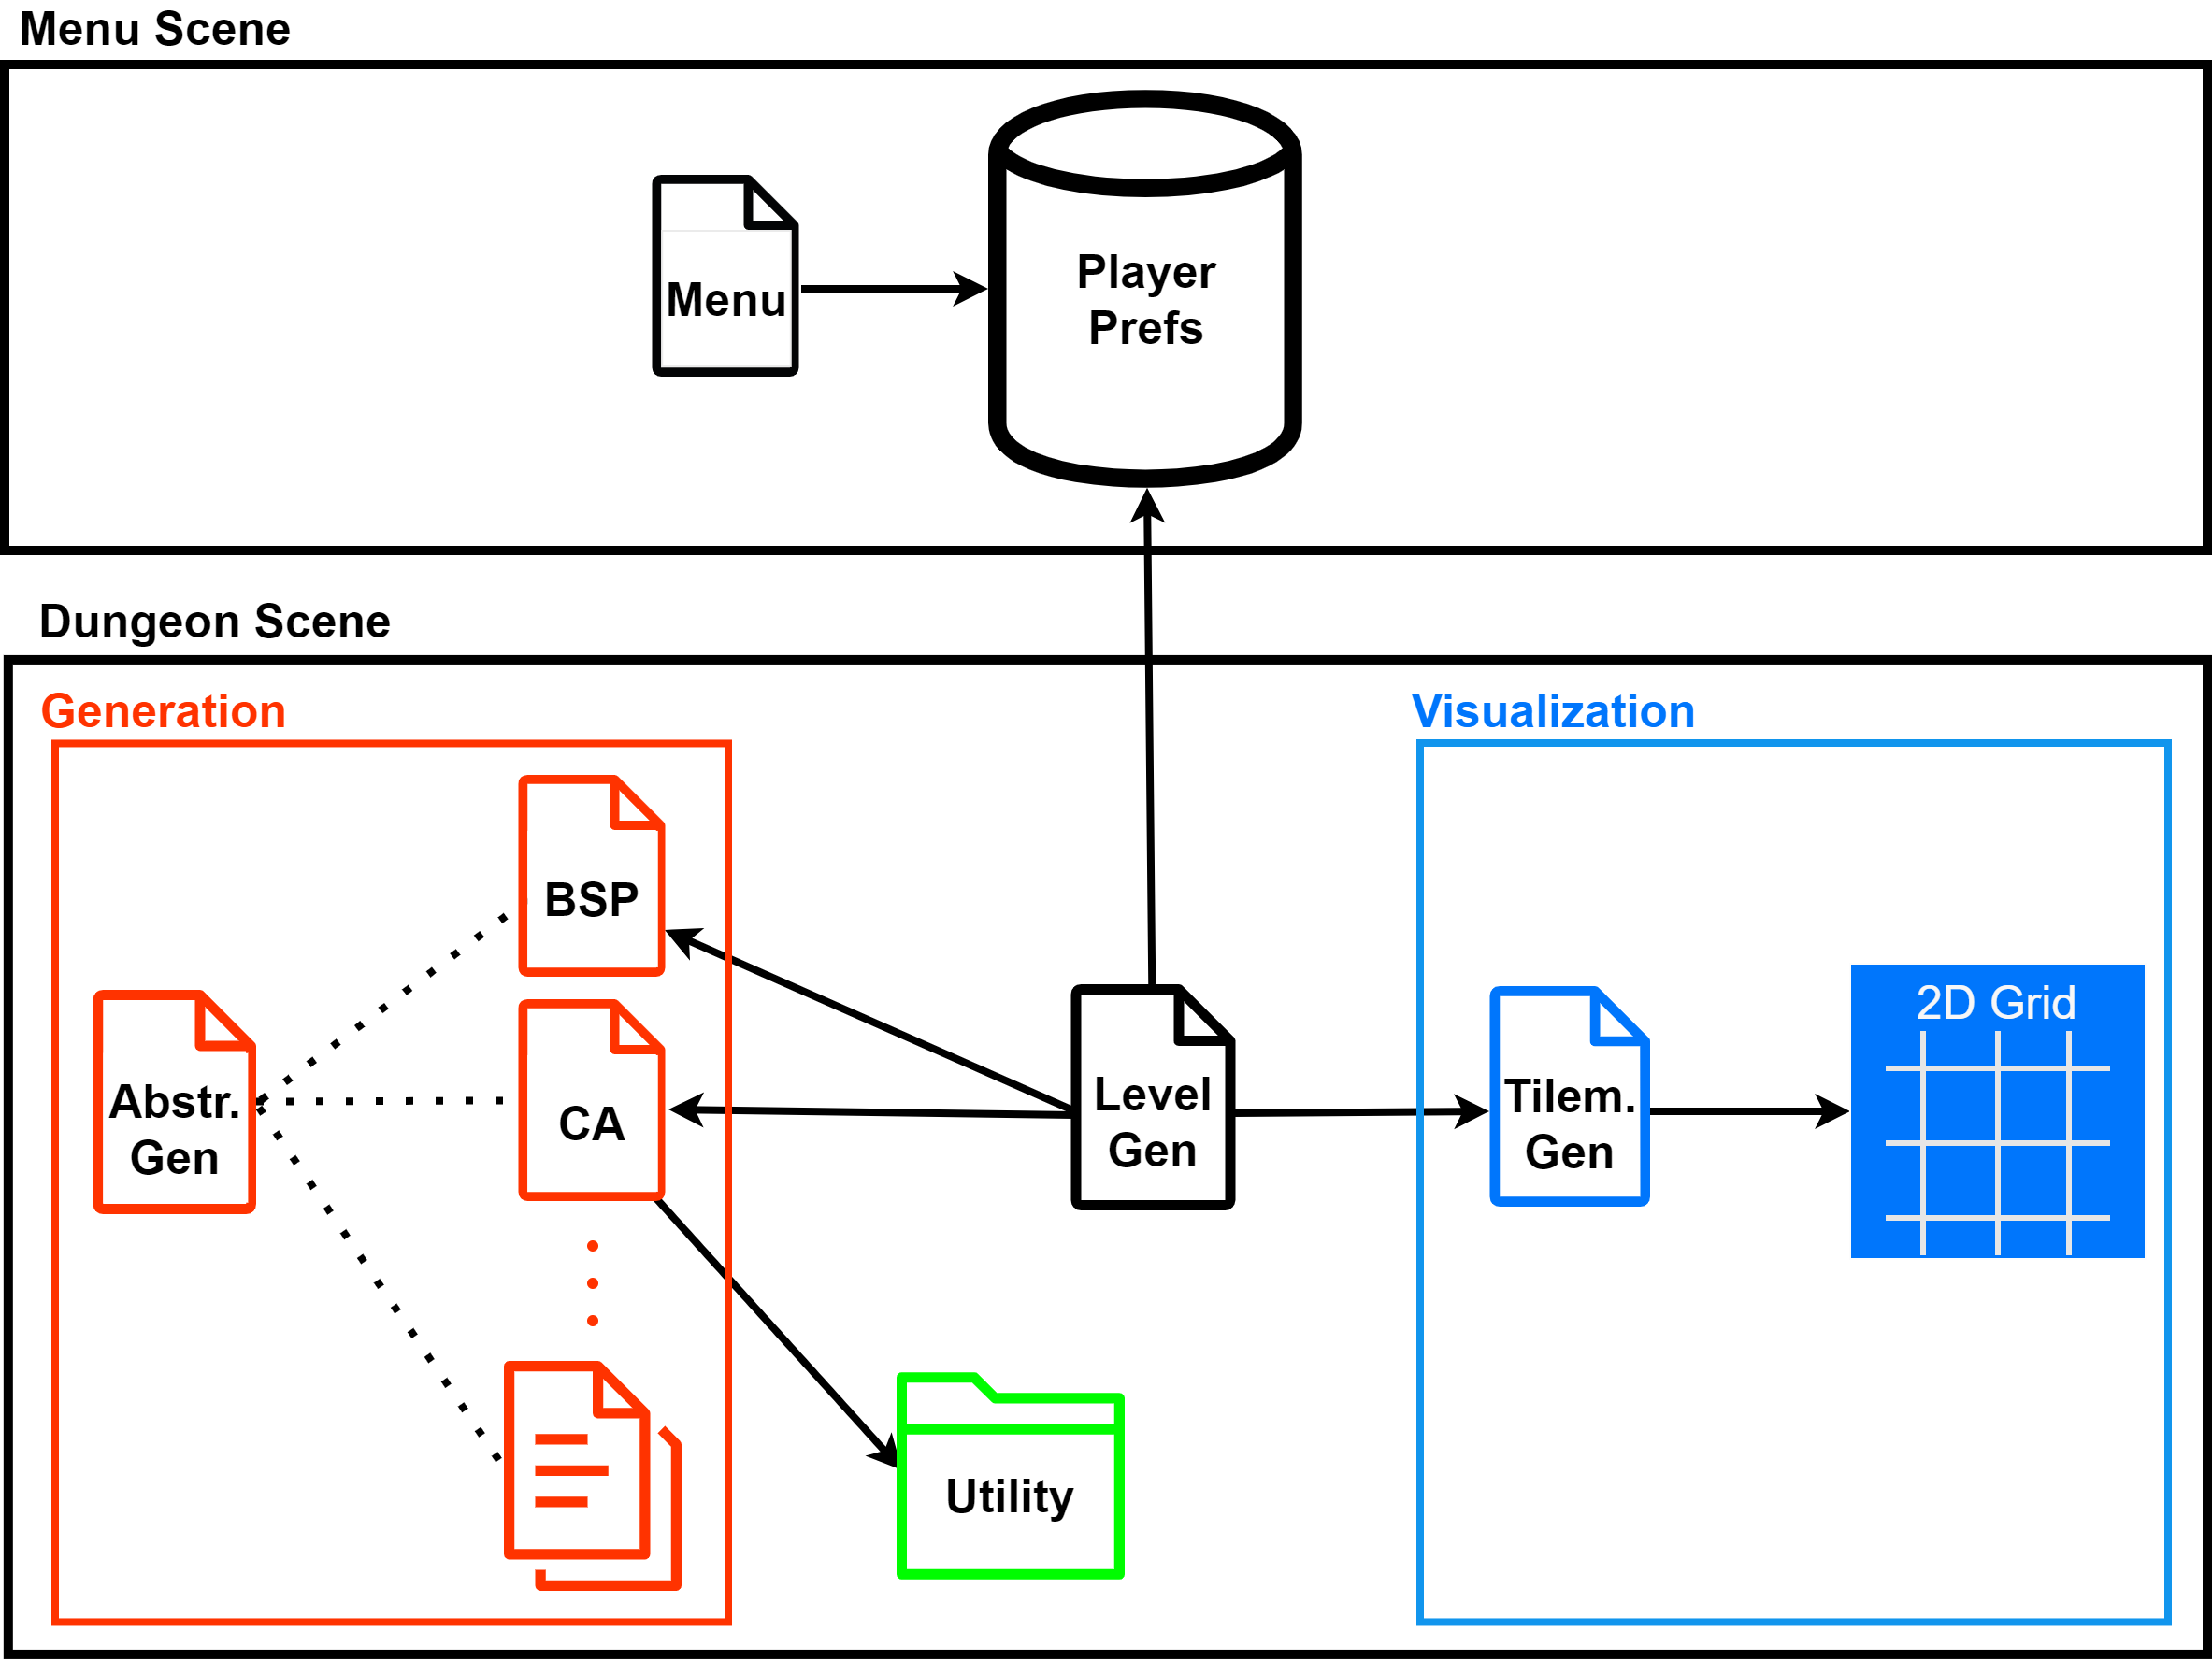
\includegraphics[width=0.8\linewidth]{obrazky-figures/scenes.png}
    \caption{Vizualizácia procesu komunikácie jednotlivých častí pri procese generovania mapy. V scéne Menu uložíme parametre generovania, v scéne Dungeon si informácie načítame, vygenerujeme požadovanou metódou mapu, ak je potrebné mapu skontrolujeme pomocnými algoritmami v zložke Utility, výslednú mapu zobrazíme na 2D mriežke}
    \label{fig:scenes}
\end{figure}

Pri vytváraní máp sme zaviedli možnosť ich generovať pomocou čísla seedu. Dosedením seedu do pseudonáhodných generátorov dostupných v Unity, dosiahneme konzistentný výsledok pri každom generovaní. Aj keď je naším cieľom vytvárať vždy nové a unikátne zážitky pre hráčov, je pre nás pri vývoji dôležité mať možnosť znovu vytvoriť chybné generácie. Navyše zdieľanie seedu a konfigurácie v komunite hráčov, ako je tomu napríklad v hre Noita, umožňuje hráčom ľahko zdieľať zaujímavé mapy, no pri každom spustení novej hry bude seed vygenerovaní náhodne a bude na hráčovi či ho bude chcieť zmeniť. S cieľom zvýšiť pohodlie hráčov sme implementovali aj funkciu prekladu písmen a znakov pri zadávaní vlastného seedu, takže môžu použiť frázu alebo vetu na nastavenie seedu pri generovaní máp.

Okrem čísla seedu a jeho nastavenia má každý generátor ďalšie spoločné charakteristiky, ako je veľkosť mapy a počiatočná inicializácia generátora. Preto sme vytvorili rozhranie \verb|AbstractGen|, z ktorého budú všetky konkrétne generátory dediť. Rozhranie poskytuje základnú štruktúru a funkcionalitu, ktorú budú ďalšie generátory využívať, čo uľahčuje a zjednodušuje ich implementáciu.

Samotné generátory implementujú jednotlivé techniky PCG, ktoré sú uvedené v kapitole \ref{sec:theory}. Výstupom každého z týchto generátorov je kolekcia hash-ov, ktorá v sebe ukladá jedinečné pozície v 2D a zabezpečuje, že sa nebudú opakovať (\verb|HashSet<Vector2D>|). Táto množina nám ponúka jednoduché a rýchle porovnávanie pozícií na 2D mriežke, čo je kľúčové pri generovaní nových pozícií mapy. Výsledná množina slúži ako základ pre generovanie stien mapy a samotnú vizualizáciu mapy. Tieto dátové štruktúry sú pre nás ideálne, pretože zabezpečujú efektívnu prácu s 2D pozíciami a prispievajú k rýchlemu a spoľahlivému generovaniu.

\subsection{Generátory}

Každý generátor má svoje vlastné nasatvenia, ktoré sa líšia. No pre zachovanie konzistencie každá mapa pracuje s rovnakým nastavením veľkosti mapy, ktorú si hráč vyberá v menu hry. Pričom ponúkame na výber malú, strednú a veľkú mapu. Malá mapa zodpovedá $35x35$ bodom mapy stredná $50x50$ a veľká $65x65$.

Pri samotnej implementácii generátorov sme postupovali podľa teórie a vedeckých článkov uvedených v kapitole \ref{sec:theory}. Keďže generátory ponúkajú rôzne konfigurovateľné parametre, vykonali sme testovanie s cieľom určiť najvhodnejšie nastavenia pre naše požiadavky. Aby bolo UI pri vytvorení 
hry prehľadné, mnohé z týchto nastavení sú pevne zvolené a prístupné výlučne v Unity editore. V prípadoch, keď výstup môže obsahovať nedosiahnuteľné oblasti, napríklad VD alebo CA, sme na overenie výslednej mapy použili algoritmom \verb|Flood| \verb|Fill|\footnote{Článok Flood Fill - \url{https://www.freecodecamp.org/news/flood-fill-algorithm-explained/}} (ďalej len FF). Ktorým všetky nedosiahnuteľné mŕtve zóny v mape sa pred vizualizáciou odstránia. Okrem toho techniky generujúce koridory obsahujú parameter šírky cesty, čo uľahčuje vytváranie širších koridorov.

\subsubsection*{Binary Space Partitioning}

Tento generátor systematicky rozdeľuje dostupný priestor na menšie obdĺžnikové miestnosti. Ak by nový priestor nedosahoval minimálnu veľkosť miestností, rozdelenie sa neuplatní a namiesto neho sa vytvorí nová miestnosť. Cyklus sa opakuje kým sa nedosiahne požadovaný počet miestností. Pri implementácii sme využili Unity typ \verb|BoundsInt|, ktorý definuje minimálne a maximálne koordináty priestoru a taktiež udržiava stred.

\noindent Nastavenia:

\begin{itemize}
    \item MinRoomSize - určuje minimálnu veľkosť miestnosti
    \item RoomCount - určuje požadovaný počet miestností
    \item Offset - udáva minimálnu vzdialenosť medzi miestnosťami
    \item CorricorWidth - určuje šírku chodieb spájajúcich miestnosti
\end{itemize}

Nakoľko je mapa štvorcová, rozdeľovanie v strede oblastí by vytvorilo predvídateľné mapy. Preto budeme náhodne vyberať medzi horizontálnym a vertikálnym rezom v náhodnom bode priestoru. K rozdeleniu dôjde jedine ak má oblasť aspoň dvojnásobok minimálnej dĺžky pre daný smer. Počet miestností je ovplyvnený aj veľkosťou mapy a je zvýšení o $2$, $3$ až $4$ miestnosti. V opačnom prípade je oblasť pridaná do zoznamu miestností a neskôr spojená koridormi, v poradí v akom boli miestnosti vygenerované (viď obr. \ref{fig:bsp}).

\begin{figure} [H]
    \centering
    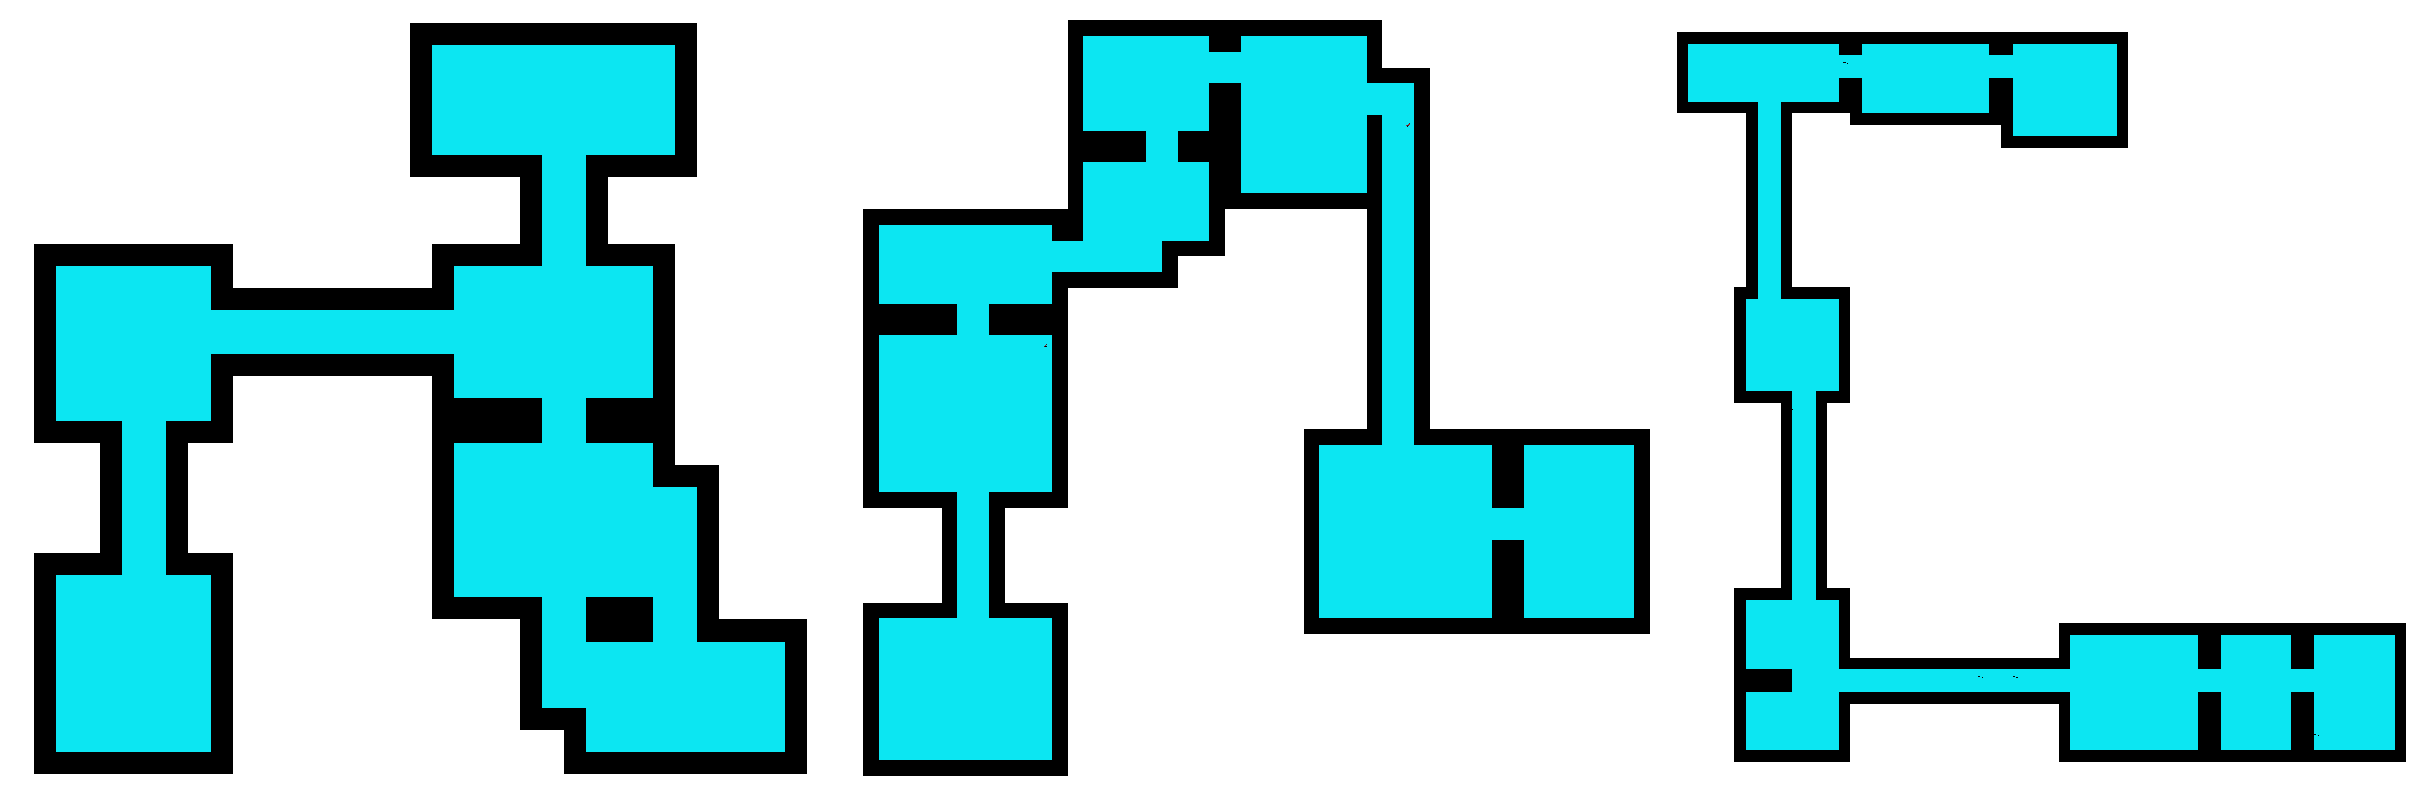
\includegraphics[width=0.75\linewidth]{obrazky-figures/bsp.png}
    \caption{Vizualizácia máp BSP, s rozličnou veľkosťou máp, so seedom $123$}
    \label{fig:bsp}
\end{figure}

\subsubsection*{Cellular Automata}

Pri procese generovania náhodne inicializujeme pole hodnotami 0 a 1 pre nevalidne a validne polia na mape. Počet valídnych polí je percentuálna hodnota z celkového počtu polí mapy. Výsledná mapa je výsledkom niekoľkých iterácií nad hodnotami poľa, podľa stanovených pravidiel a okolitého susedstva. Na konci je pole skontrolované FF a prevedené na hashový set.

\noindent Nastavenia:

\begin{itemize}
    \item PercentCoverage - určuje percento mapy, ktoré je na začiatku pokryté dlaždicami
    \item Iterations - nastavuje počet iterácií nad 2D poľom
    \item ShowValid - zapína / vypína vizualizáciu nedostupných častí mapy
\end{itemize}

\begin{figure} [b]
    \centering
    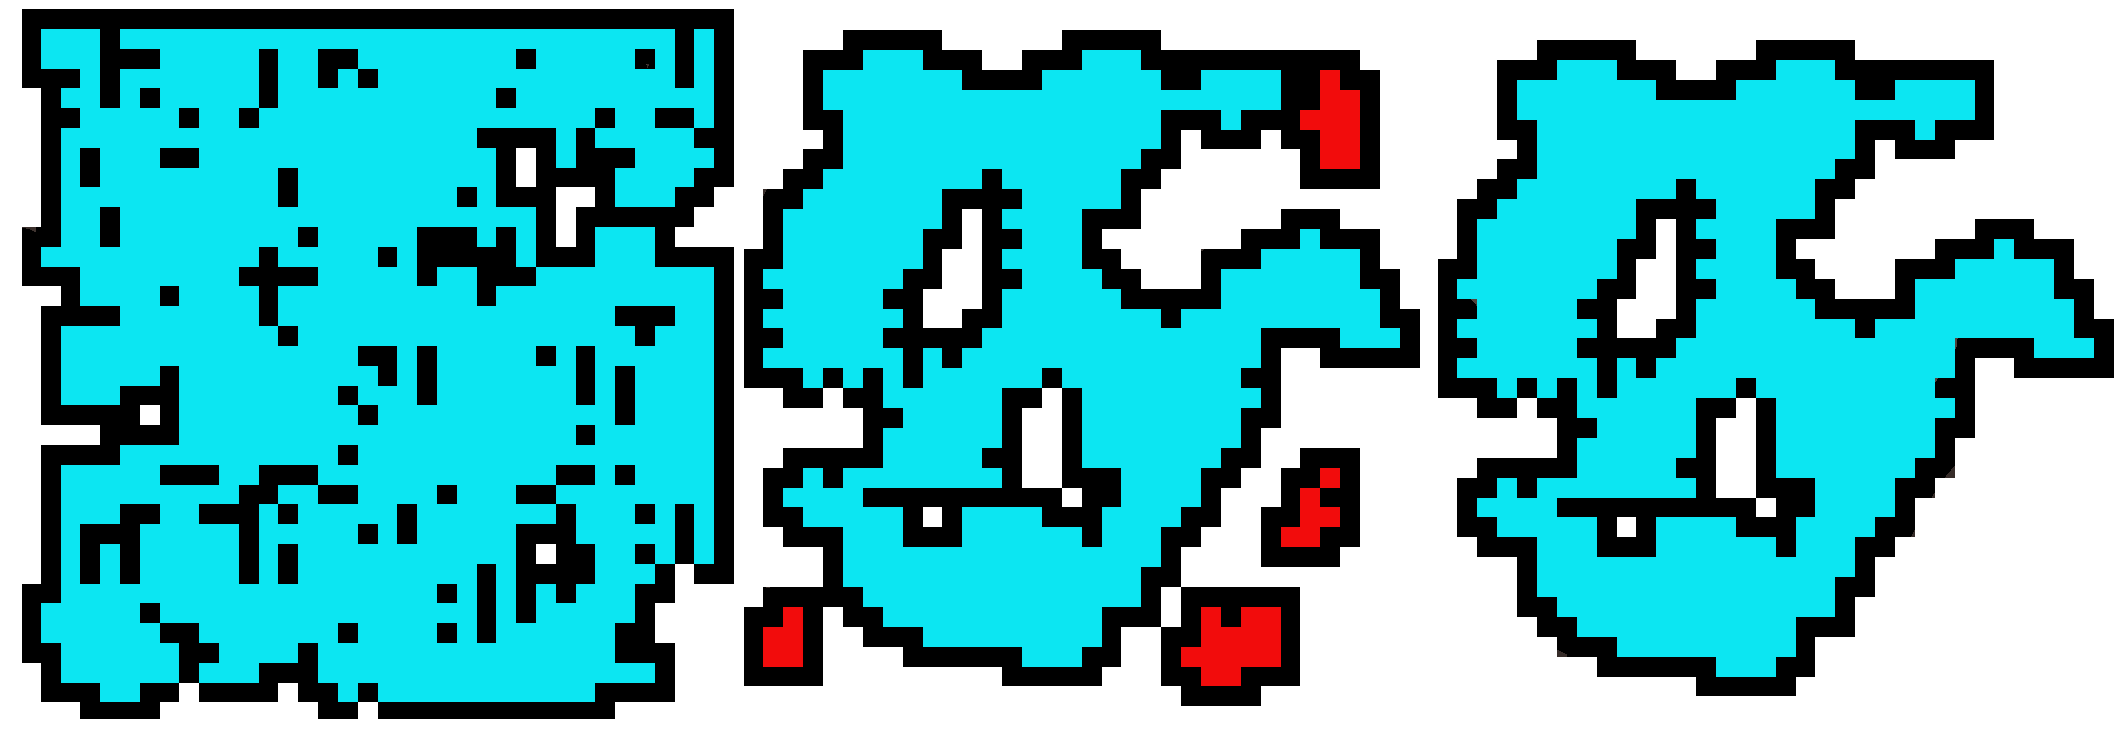
\includegraphics[width=0.75\linewidth]{obrazky-figures/ca.png}
    \caption{Postupná vizualizácia mapy CA, zľava doprava 0. iterácia, 4. iterácia, vymazanie mŕtvych častí pomocou FF}
    \label{fig:ca}
\end{figure}

Pri implementácii pravidiel sme testovaním zistili, že pre naše potreby najlepšie vyhovuje Moorovo okolie bunky a do novej iterácie mapy zapíšeme iba tie body ktoré majú viac ako $4$ susedov. Dovoľuje nám to nastaviť vyššie percento existujúcich bodov v počiatočnom stave mapy a každou iteráciou mažeme časti mapy. Preto budeme o tomto pravidle hovoriť ako o mazacom. 
Opačným pravidlom by sme zapisovali do novej mapy body s menej ako $4$ susedmi (viď obr. \ref{fig:ca}). Takéto pravidlo však môže rýchlo naplniť celú mapu alebo vytvára nespojené ostrovy ak by sme znížili počet bodov v počiatočnom stave. Ďalšie variácie pravidiel zohľadňujúce konkrétne pozície susedov, iné typy susedstva napr. Von Neumannovo, alebo kombinácie mazacích a pridávajúcich pravidiel, sa nám neosvedčili.

\subsubsection*{Diamond Square}

Inicializujeme prázdne 2D pole, jeho rohom náhodne priradíme hodnotu od 0 do veľkosti mapy. Následne iteratívne generujeme výškové hodnoty koordinátor na mape, vykonávaním kombinácie diamantových a štvorcových krokov. 

\noindent Nastavenia:

\begin{itemize}
    \item Roughness - určuje drsnosť alebo hladkosť terénu
    \item Threshold - stanovuje prahovú hodnotu od ktorej považujeme pozíciu za dlaždicu mapy
    \item ShowValid - zapína / vypína vizualizáciu nedostupných častí mapy
\end{itemize}

Výsledný generátor je však obtiažne nastaviť pre naše potreby. V 2D prostredí vytvára mnoho odpadu v podobe nedostupných častí mapy, jeho najvhodnejšie využitie by bolo pre tvorbu močiarov / ruín kde by hráč vedel veľmi časté jednodlaždicové medzery vypĺňať (viď obr. \ref{fig:ds}).   

\begin{figure} [H]
    \centering
    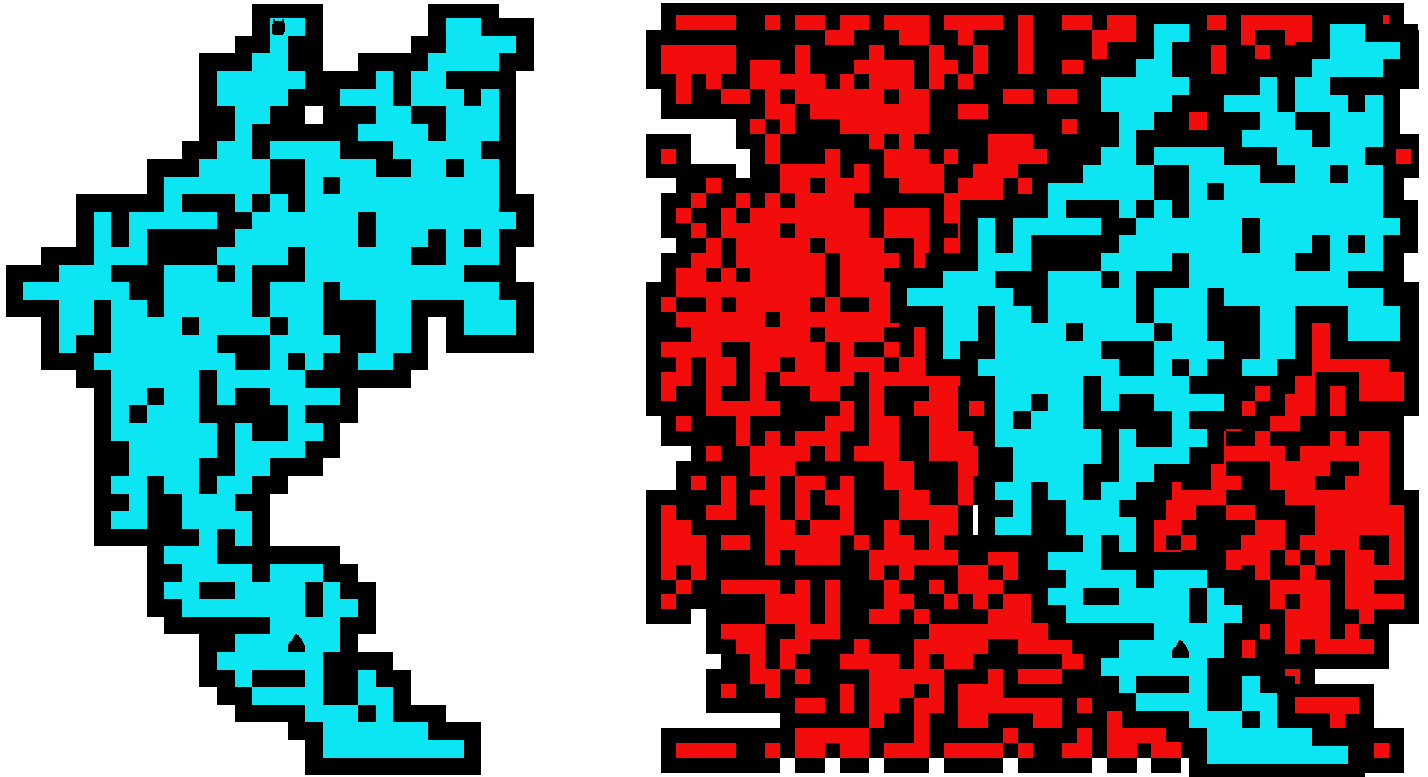
\includegraphics[width=0.5\linewidth]{obrazky-figures/ds.png}
    \caption{Vizualizácia mapy DS, červená je nedostupná časť mapy, odstránená FF}
    \label{fig:ds}
\end{figure}

\subsubsection*{Diffusion Limited Aggregation}

Pri generovaní simulujeme rast častíc v ohraničenom priestore, pričom častice sa časom spájajú. Proces vytvára agentov na hraniciach mapy, ktorý sa náhodne pohybujú priestorom. Ak by agent vyšiel za hranice mapy je zmazaný a vytvorí sa na jeho mieste nový. 

V rámci implementácie sme vytvorili možnosť generovať z hraníc štvorca alebo kružnice s priemerom veľkosti mapy a s centrálnym ťažiskom. Ak generujeme s centrálnym ťažiskom je $50\%$ šanca, že sa agent priblíži k cieľu.

\noindent Nastavenia:

\begin{itemize}
    \item PercentCoverage - určuje percentuálne pokrytie rozlohy mapy dlaždicami
    \item Central - zapne/vypne náhodné ovplyvňovanie smeru agenta k centru mapy
    \item CentralChance - percentuálna šanca resp. váha ťažiska, ktorá ovplyvní výber smeru k centru ak je zapnuté nastavenie Central
    \item Cirle - určuje vznik agentov na kružnici alebo štvorcových hraniciach
\end{itemize}

\begin{figure} [H]
    \centering
    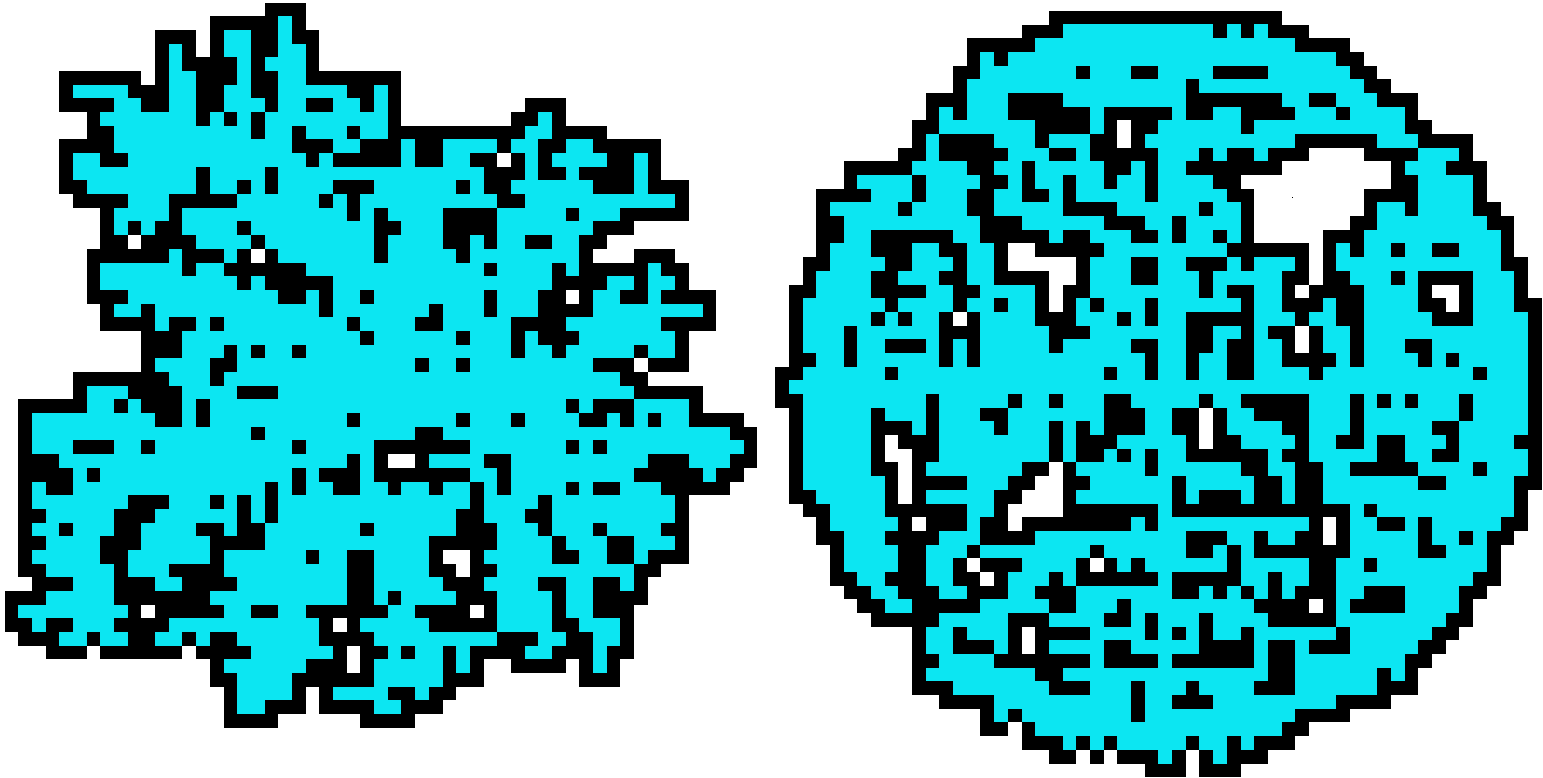
\includegraphics[width=0.6\linewidth]{obrazky-figures/dfa.png}
    \caption{Vizualizácia mapy DFA bez ťažiska, seed $123$, zo štvorca vľavo, z kružnice vpravo}
    \label{fig:dfa}
\end{figure}

Pre naše potreby budeme využívať generovanie na kruhu bez ťažiska. Generovanie s ťažiskom vytvára otvorený stred a uberá detaily na okrajoch mapy. Našim cieľom je aby hráč prešiel väčšinu mapy, preto je vhodné aby boli hranice mapy otvorenejšie ako jej stred. 

Generovanie zo štvorca vytvára vetvy medzi ktorými nie je prechod. Bez ďalších úprav by takáto mapa nútila hráča často prechádzať stredom aby preskúmal každú z nich (viď obr. \ref{fig:dfa}).

\subsubsection*{Generatívna Gramatika}

Pri generovaní využívame proces rozširovania reťazca znakov. Naša definovaná gramatika obsahuje terminálne a neterminálne znaky. Každý neterminálny znak bude nahradený terminálnym a náhodným generovaním rozšírený o ďalší znak. Aby bol proces generovania konečný, môžeme ho obmedziť počtom iterácií, počtom miestností, alebo nižšou šancou na rozšírenie o neterminálne znaky. 

Pre naše potreby potrebujeme miestnosti, označenie začiatku, konca dungeonu a koridorov ktoré môžu meniť smer. Určíme si znaky S a E ako štartovaciu a konečnú pozíciu, S/E/B/b označujú miestnosť, c/C koridor ktorý pokračuje v danom smere, r/R zmenu smeru vpravo, l/L vľavo a koridor v novom smere. 

\noindent Množiny znakov a pravidiel:

$$    \textnormal{Množina všetkých znakov : }\;V = \{ S, C, R, L, B, E, c, r, l, b \} $$
$$    \textnormal{Množina terminálov : K}\; = \{ S, C, R, L, B, E\} $$
$$    \textnormal{Množina neterminálov : N}\; = \{ c, r, l, b \} $$
$$    \textnormal{Pre}\;\forall\;x \in N\;\textnormal{platí, že}\;\exists\;y \in K $$
$$    \textnormal{Funkcia :} f(x) = y;\;\textnormal{mapuje}\;x \in N\;\textnormal{na}\;y \in K $$
$$    \textnormal{Funckia :}\;h()\;\textnormal{ vracia náhodný znak z množiny} K $$
$$    \textnormal{Funckia :}\;g()\;\textnormal{ vracia náhodný znak z množiny} N $$
$$    \forall\;x \in N \Rightarrow \Bigg\{ \begin{array}{c c} 
         f(x) + h() & s\;pravdepodobnosťou\;60\%\\ 
         f(x) + g() & s\;pravdepodobnosťou\;40\%\\ 
      \end{array} $$ 
$$    \textnormal{Počiatočný reťazec :}\;Scb + cbc * MapSize + lcE; MapSize \in \{1, 2, 3\} $$

\newpage
\noindent Nastavenia:

\begin{itemize}
    \item MinCorLen / MaxCorLen - určujú minimálnu a maximálnu dĺžku koridorov
    \item MinRoomSize / MaxRoomSize - určuje minimálnu a maximálnu veľkosť miestností
\end{itemize}

\noindent Táto gramatika generuje reťazec, v ktorom sú produktívne symboly nahradené a rozšírené o ďalšie symboly podľa pravidiel. Podľa výsledného reťazca vygenerujeme konečnú podobu dungeonu. Výsledný generátor sa ukázal ako spoľahlivý zvlášť pre malé mapy (viď obr. \ref{fig:gg}).

\begin{figure} [H]
    \centering
    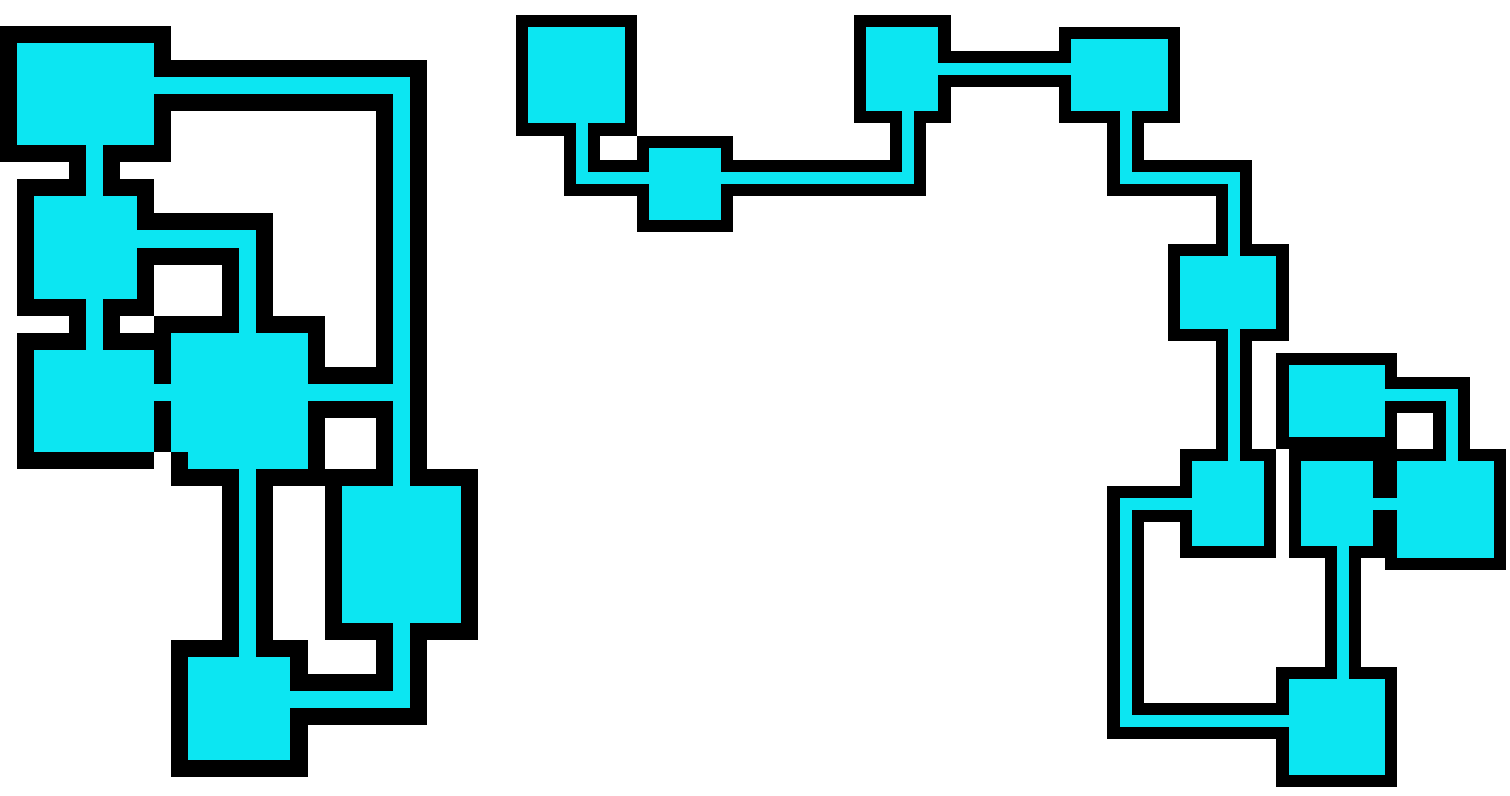
\includegraphics[width=0.47\linewidth]{obrazky-figures/gg.png}
    \caption{Vizualizácia mapy generatívnej gramatiky, veľkosť mapy vľavo malá, vpravo veľká}
    \label{fig:gg}
\end{figure}

\subsubsection*{Perlin Noise}

Tento generátor tvorí šum s viacerými oktávami, čo umožňuje vytvárať zložitejšie a podrobnejšie vzory. Pre každú oktávu taktiež generujeme náhodný posun od počiatku na základe seedu, bez posunov by každá oktáva začínala v rovnakom bode, čo by viedlo k opakujúcim sa vzorom. Parametre ako perzistencia a lakunarita riadia ďalšie vlastnosti šumu a využívame ich na zmenu amplitúdy a frekvencie pri výpočte konkrétnej oktávy. Pre samotný výpočet hodnoty Perlinovho šumu využívame zabudovanú funkciu \verb|PerlinNoise| z balíka \verb|Mathf|. Takto vypočítané hodnoty porovnávame voči prahovej hodnote a vyhovujúce body sú zapísané do mapy. Posledným krokom je využitie FF na odstránenie nedosiahnuteľných častí mapy.

\noindent Nastavenia:

\begin{itemize}
    \item Persistence - hodnota v rozsahu $0.1$ až $1$ určuje ako rýchlo sa znižuje amplitúda pre každú nasledujúcu oktávu
    \item Lacunarity - hodnota v rozsahu $1$ až $3$ určuje ako rýchlo sa zvyšuje frekvencia pre každú nasledujúcu oktávu
    \item Octaves - určuje počet oktáv, vyšší počet oktáv vytvára detailnejšie vzory
    \item Threshold - prahová hodnota rozhodujúca od akej hodnoty považujeme body ako dlaždice mapy
    \item ShowValid - zapína / vypína vizualizáciu nedostupných častí mapy 
\end{itemize}

Ďalšie parametre ovplyvňujúce generovanie sme testovaním nastavili tak aby sme boli spokojný s výslednými mapami. Napríklad pre škálovanie používame veľkosť mapy násobenú $5\times$. Náhodný Posun oktávy je z rozsahu $\left<-10\,000; 10\,000\right>$. Amplitúda a frekvencia začína na hodnote $1$. A jednotlivé hodnoty oktáv pre jeden bod delíme počtom oktáv pre normalizovanie hodnôt. Testovaním sme si určili ideálnu detailnosť mapy pri $6$ oktávach a prah $0.15$ (viď obr. \ref{fig:pn}).

\begin{figure} [H]
    \centering
    
\includegraphics[width=0.77\linewidth]{obrazky-figures/pn.png}
    \caption{Vizualizácia mapy Perlinovho šumu, zľava doprava $4$, $5$ a $6$ oktáv}
    \label{fig:pn}
\end{figure}

\subsubsection*{Simple Room Placement}

Pri generovaní mapy začíname náhodným umiestnením miestností v hraniciach mapy. Počet miestností sa skladá z pevne definovaného počtu a dynamicky získaného počtu, ktorý závisí od veľkosti mapy ($3$ až $6$). Koordináty stredov miestností sa uložia do listu. Iteráciou nájdeme najbližší stred ďalšej meistnosti a spojíme ich koridorom. Koridory vytvárame jednoduchým porovnávaním aktuálnej a cieľovej pozície na X a Y súradniciach. Úpravou týchto nastavení vieme vytvoriť vždy originálne rozvrhnutie dungeonov.

\noindent Nastavenia:

\begin{itemize}
    \item MinRoomSize / MaxRoomSize - určuje minimálnu a maximálnu veľkosť miestností
    \item RoomCount - určuje počet miestností
    \item Offset - určuje minimálnu vzdialenosť medzi miestnosťami
    \item CorridorWidth - určuje šírku chodieb spájajúcich miestnosti
\end{itemize}

\begin{figure} [H]
    \centering
    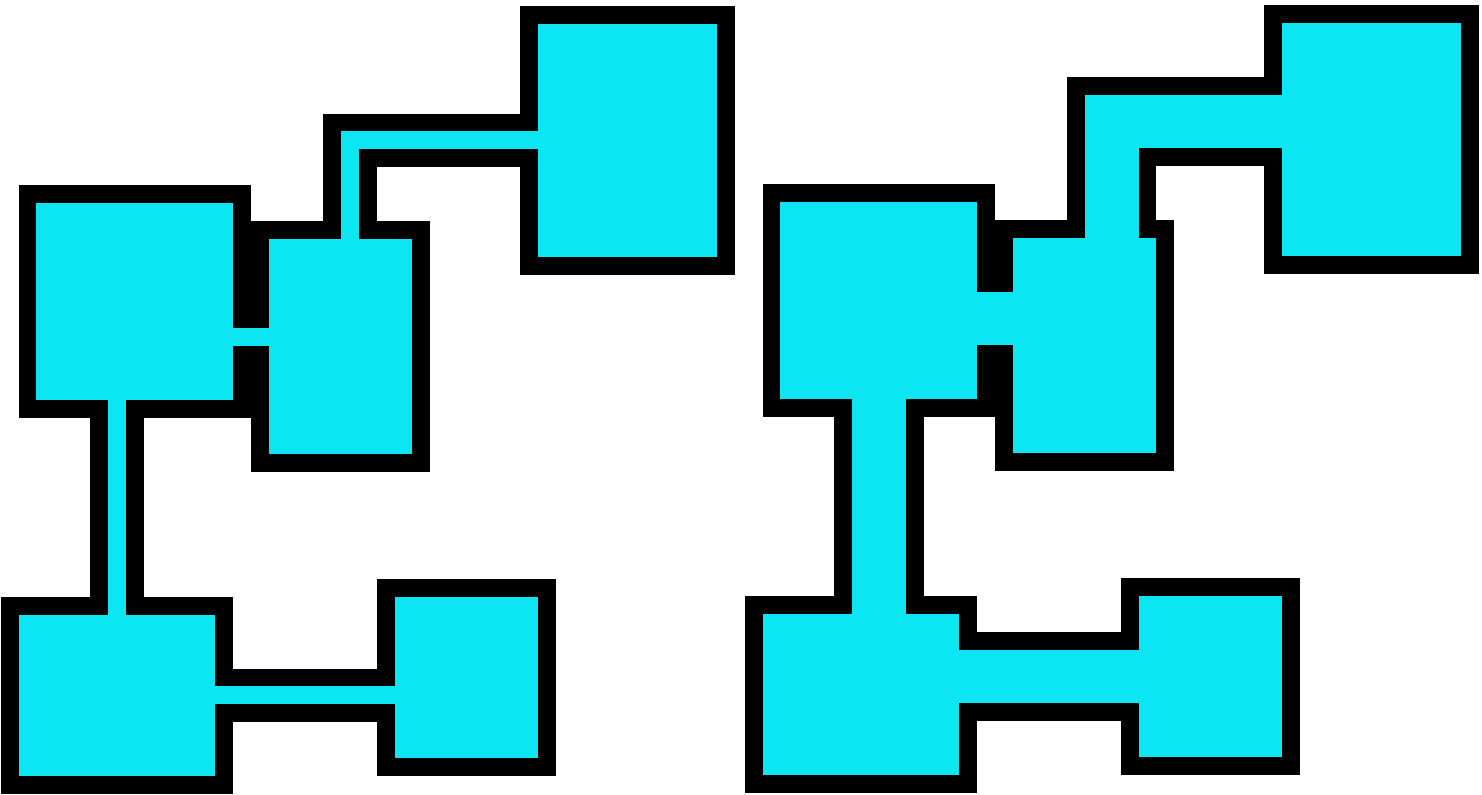
\includegraphics[width=0.47\linewidth]{obrazky-figures/srp.png}
    \caption{Vizualizácia mapy SRP, so zmenou šírky koridorov $1$ vľavo $3$ vpravo}
    \label{fig:srp}
\end{figure}

\subsubsection*{Random Walk}

Tento generátor je implementovaný pomocou náhodného pohybu agentov. Proces začína vytvorením koridorov a uchovaním ich koncových bodov do listu potenciálnych stredov miestností. V závislosti na veľkosti mapy vyberieme $18\%$, $25\%$ alebo $33\%$ bodov z listu a generujeme na nich miestnosť. Následne zistíme ktoré nepoužité body z listu sú súčasne slepé uličky a vygenerujeme v týchto bodoch miestnosť.

\noindent Nastavenia:

\begin{itemize}
    \item CorridorIter - určuje počet iterácií a teda aj počet koridorov
    \item CorridorLen - určuje počet krokov v iterácii a teda aj dĺžku jedného koridoru
    \item CorridorWalkBack - dovoľuje pri generovaní koridorov vrátiť sa v smere z ktorého prišli
    \item RoomIter - určuje počet iterácií ktorými generujeme miestnosť
    \item RoomLen - určuje počet krokov v jednej iterácii 
    \item RandomiseRoomStartPos - dovoľuje náhodný výber novej pozície pri každom kroku v iterácii
    \item MapBounds - dovoľuje / zakazuje presah za hranice mapy
\end{itemize}

Pri generovaní koridorov, na začiatku iterácie vyberieme náhodný kardinálny smer ktorým koridor pôjde. Ak narazíme na hranice mapy a je zakázané ísť za ne, zmení sa tento smer o $90^\circ$ vľavo. Ak by vygenerovaný smer bol opačný k doterajšiemu, a nie je povolený \verb|CorridorWalkBack| zmení a o $90^\circ$ vpravo. Pri generovaní miestností sa smer náhodne mení každým krokom, rovnako ako pri koridoroch, ak by mala byť nová pozícia mimo hranice a nie je to dovolené, smer sa zmení o $90^\circ$ vpravo. Výber smeru otočenia o $90^\circ$ nie je dôležitý. Pri testovaní sme však najlepšie výsledky dosiahli pri povolení presahu dlaždíc za hranice mapy. Generujeme tak proporčne väčšie mapy ako u iných generátorov no výsledky sú lepšie. 

\begin{figure} [H]
    \centering
    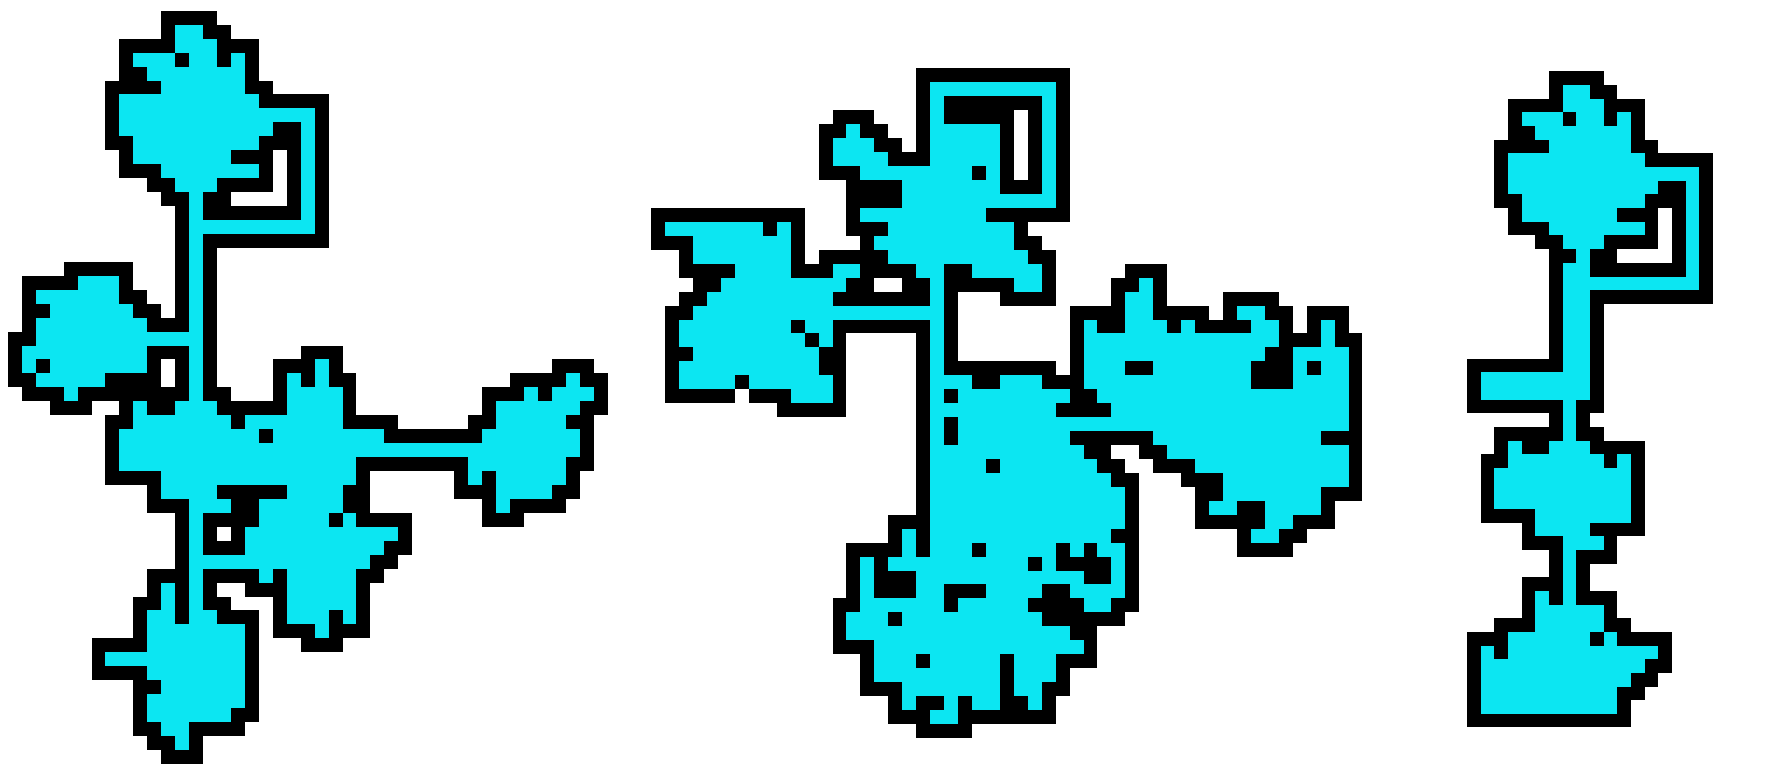
\includegraphics[width=0.65\linewidth]{obrazky-figures/rw.png}
    \caption{Vizualizácia mapy RW, seed 123, vľavo štandardné generovanie, v strede povolenie \texttt{RandomiseRoomStartPos}, vpravo zákaz \texttt{MapBounds}}
    \label{fig:enter-label}
\end{figure}

\subsubsection*{Voronoi Diagram}

Na začiatku procesu inicializujeme prázdne 2D pole, na náhodných miestach rozložíme semienka s rozličnými hodnotami. Pre každý bod na mape vypočítame jeho najmenšiu vzdialenosť k jednému zo semiačok ku ktorému je následne priradené, zmenou hodnoty na hodnotu daného semiačka. Namiesto bežného využitia tejto techniky na generovanie území, sme využili práve hranice medzi nimi ako koridory (viď obr. \ref{fig:vd}). Následne na ich koncoch generujeme potrebný počet miestností. Využitím \verb|A*| získame najkratšie cesty medzi miestnosťami, nevyužité koridory sú vymazané.

\noindent Nastavenia:

\begin{itemize}
    \item DistanceMethod - možnosť výberu metódy použitej na výpočet vzdialenosti semiačok, môžeme si vybrať medzi Euklidovskou a Manhattanskou vzdialenosťou
    \item MinRoomSize / MaxRoomSize - určuje minimálnu a maximálnu veľkosť miestností
    \item VoronoiSeeds - určuje počet semiačok
    \item RoomCount - určuje požadovaný počet miestností
    \item Offset - udáva minimálnu vzdialenosť medzi miestnosťami
    \item ShowValid - zapína / vypína vizualizáciu nedostupných častí mapy
\end{itemize}

\begin{figure} [H]
    \centering
    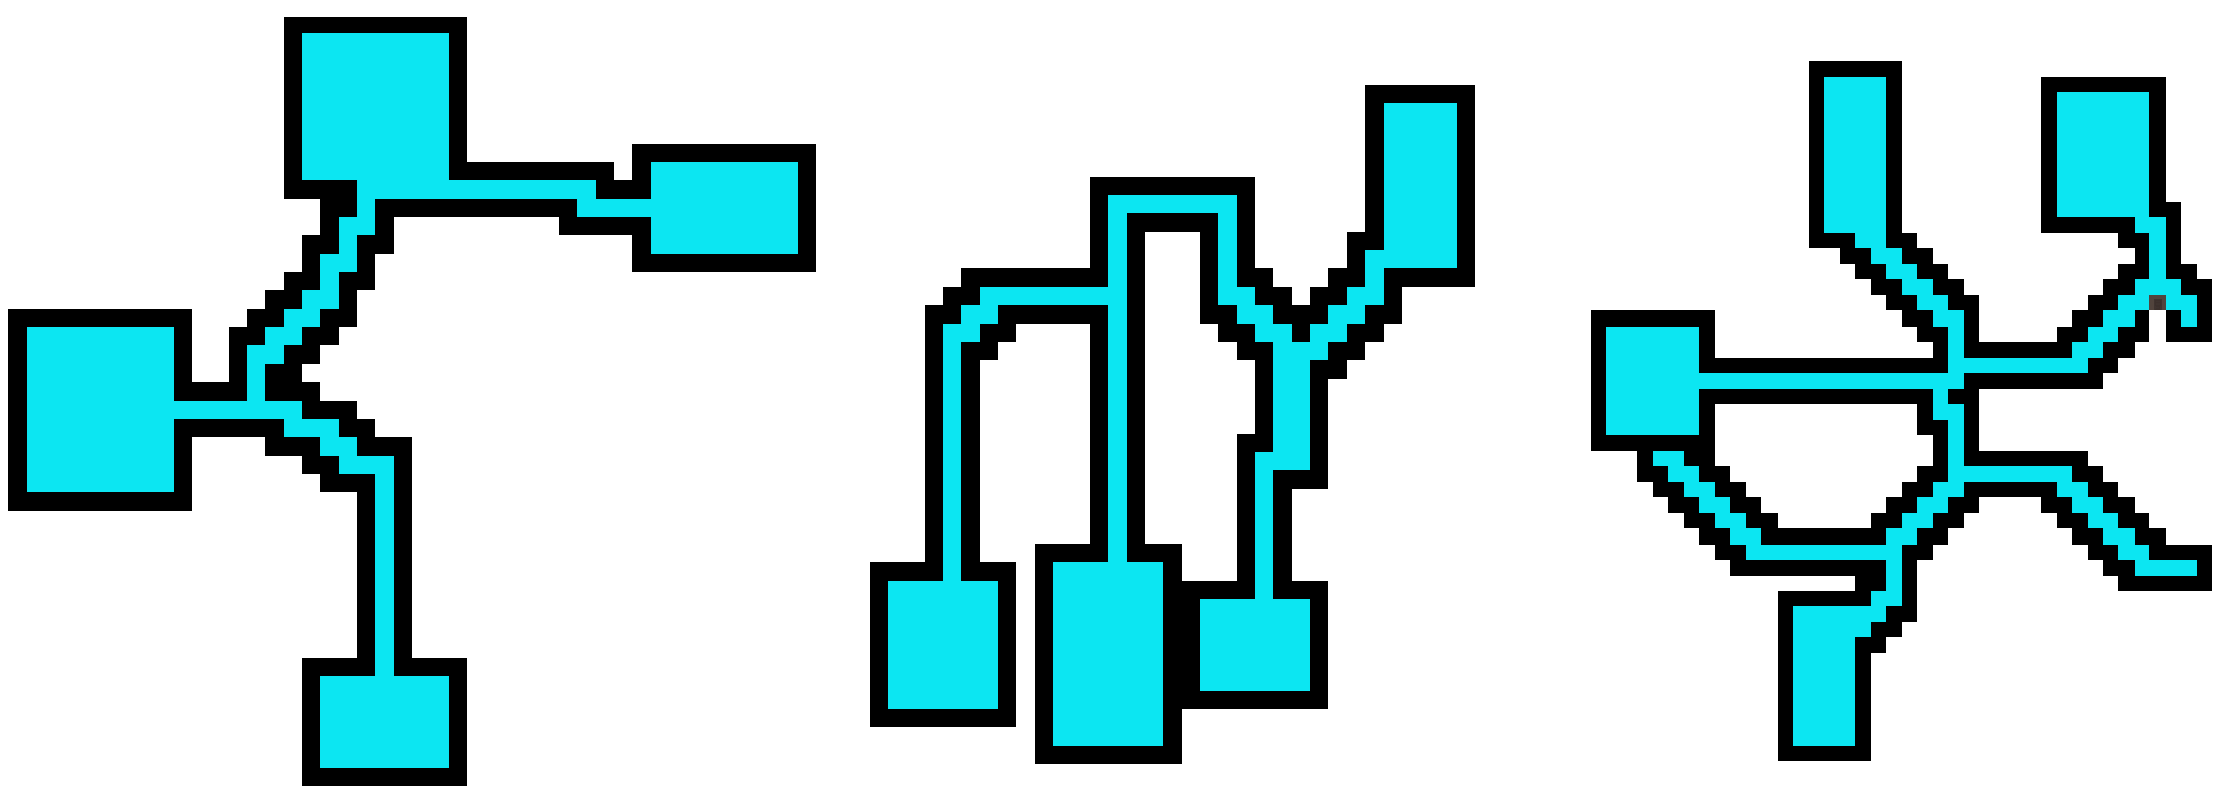
\includegraphics[width=0.7\linewidth]{obrazky-figures/vd.png}
    \caption{Vizualizácia mapy VD, vľavo s Euklidovou, v strede s Manhatanovou vzdialenosťou, vľavo nevyčistená mapa}
    \label{fig:vd}
\end{figure}

\subsection{Generovanie stien}

Na obmedzenie pohybu hráča v rámcoch vygenerovanej mapy používame kompozitný collider pre dlaždicové mapy (\verb|Tilemap|\verb|Collider|\verb|2D|, \verb|Composite|\verb|Collider|\verb|2D|). Ktorý spája jednotlivé steny do uceleného collideru. Tým sa detekcia kolízií stáva efektívnejšou, pretože musíme vyhodnocovať len kolízie s väčšími hranami stien, a nie s každým jednotlivým malým blokom. Aby sme zvýšili vizuálnu príťažlivosť, v našej hre sú steny v kardinálnych aj diagonálnych smeroch. Spolu máme 10 grafických reprezentácií stien ktorých použitie dynamicky generujeme na základe okolia. Binárnym kódovaním okolia každej steny zistíme akú grafickú variantu potrebujeme. Proces sme rozdelili do troch častí:

\begin{enumerate}
\item Detekcia stien - prechádzaním všetkých bodov na mape a hľadaním dostupných susedov v kardinálnych aj diagonálnych smeroch
\item Bitové kódovanie - vytvorenie 4-bitových jednoduchých stien a 8-bitových zložitých stien, kde počet bitov zodpovedá počtu okolitých blokov
\item Vizualizácia - výber vhodnej grafiky na základe bitového kódovania
\end{enumerate}

Tento proces sa vykoná samostatne najprv pre jednoduché steny nachádzajúce sa v kardinálnych smeroch a následne pre komplexné steny nachádzajúce sa aj na diagonálne (viď obr. \ref{fig:bit-walls}). Rôzne bitové kombinácie pre každú situáciu sme vložili do triedy \verb|WallBitValues|.

\begin{figure} [H]
    \centering
    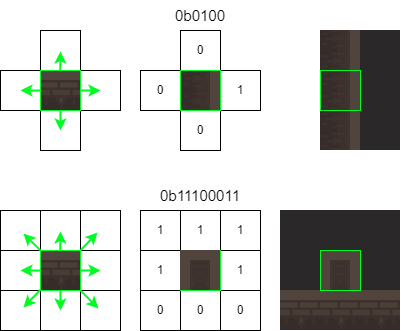
\includegraphics[width=0.6\linewidth]{obrazky-figures/bit-walls.png}
    \caption{Vizualizácia procesu kódovania stien, najprv kódujeme jednoduché steny v 4 smeroch (horná polovica), následne komplexné steny v 8 smeroch (dolná polovica), kódovanie začína v smere nahor a postupuje v smere hodinových ručičiek, 0 - prázdne / nepriechodné políčko mapy, 1 - priechodné políčko mapy}
    \label{fig:bit-walls}
\end{figure}

\subsection{Generovanie nepriateľov}

Posledným krokom pri generovaní mapy je umiestnenie začiatočného a konečného bodu. Vzdialenosť medzi nimi je minimálne $65\%$ šírky mapy a pomocou \verb|A*| algoritmu sa overí, že medzi bodmi existuje cesta. Následne na mape náhodne generujeme nepriateľov. Je možné generovať z niekoľkých typov, pričom je šanca pre daný typ rovnomerne rozdelená. Aby sme umožnili hráčom sťažiť si hru, ponúkame $4$ úrovne obtiažnosti a $3$ herné kolá, pričom obe tieto premenné zvyšujú počet nepriateľov na mape. Počet nepriateľov potom získame: $\textnormal{obtiažnosť} \times 15 + \textnormal{kolo} \times 5 + 25$. Aby nebol hráč hneď po načítaní mapy pod útokom, sú nepriatelia generovaný v minimálnej vzdialenosti $8$ blokov.

\begin{figure} [H]
    \centering
    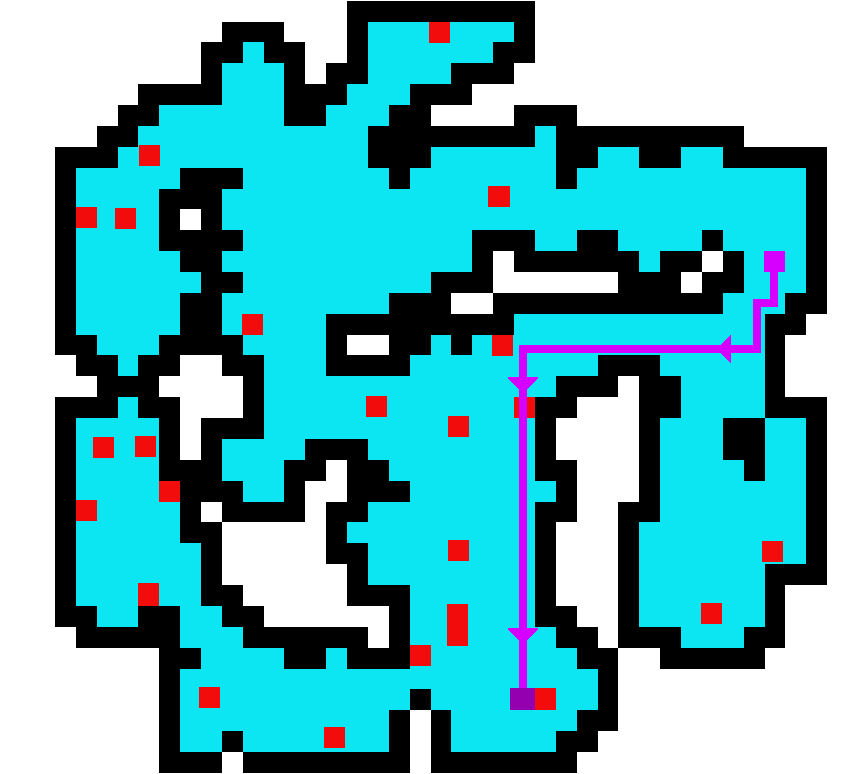
\includegraphics[width=0.45\linewidth]{obrazky-figures/enemies.png}
    \caption{Vizualizácia mapy, červená farba predstavuje nepriateľov, fialové body štart a konečný bod, fialová cesta je najkratšia cesta nájdená \texttt{A*}}
    \label{fig:enemies}
\end{figure}

\section{Herné mechaniky}

Pri konečnej implementácii sme sa zamerali na vytvorenie škálovateľných systémov. Vo finálnej verzii hry sme sa prioritne zamerali na položenie základov týchto systémov ako je pathfinding, kontextové riadenie, UI navigácia, systém schopností a postavy. Tieto systémy poskytujú základ, na ktorom možno v budúcich iteráciách hry budovať ďalšie funkcie a vylepšenia. 

\subsection{Hráč}

Do hry sme implementovali pohyb hráča pomocou štandardných kláves \verb|W| \verb|A| \verb|S| \verb|D|. Ďalej mechaniku posadnutia, vďaka ktorej môžu hráči posadnúť nepriateľov a golemov. Výnimkou sú bossovia na konci každej úrovne. Hráč má vlastné životy, no ak má kontrolu nad iným telom, preberá životy aj schopnosti danej postavy, ktorá dostane všetko poškodenie namiesto hráča (viď obr. \ref{fig:spellbar}).

Hráč posadne postavu presunutím myšky nad cieľ a stlačením medzerníku. Pri tomto procese sa overí niekoľko vecí (viď obr. \ref{fig:possess-example}):

\begin{itemize}
    \item Získame prvý objekt v okolí kurzoru, ktorý patrí do skupiny posadnuteľných objektov
    \item Ak je už hráč v objekte, kontaktuje ho a následne kontaktuje nový objekt
    \item Vymenia sa schopnosti, referencie na vizualizáciu životov, objektu sa označí ako hráč a originálnemu hráčovi (duchovi) vypneme jeho collider a grafiku.
\end{itemize}

V tejto verzii hry netrestáme pri preskakovaní medzi postavami a kvôli ďalšiemu testovaniu s touto mechanikou sme ponechali aj možnosť posadnúť postavy cez steny. Aj keď podobný systém detekovania hráča cez steny alebo vyskočenie ducha za hranice mapy, je zakázaný. Obdobným spôsobom môže hráč objekt opustiť, pri dlhšom stlačení medzerníku a objaví sa na mieste kurzoru. Ak je po ceste ku kurzoru detekovaná stena, hráčova nová poloha bude tesne pred jej začiatkom. Ak hráč pustí medzerník priskoro a v dosahu budú nepriatelia, presunieme ho do náhodného z nich.

\begin{figure} [H]
    \centering
    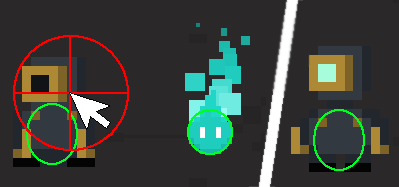
\includegraphics[width=0.75\linewidth]{obrazky-figures/possess-example.png}
    \caption{Vizuálny príklad posadnutia a grafická zmena po jeho dokončení}
    \label{fig:possess-example}
\end{figure}

\begin{figure} [H]
    \centering
    
\includegraphics[width=0.75\linewidth]{obrazky-figures/spellbar.png}
    \caption{Vizualizácia UI pre hráčove životy (vľavo) a životy posadnutého objektu (vpravo), schopnosti a aktívny cooldown (v strede)}
    \label{fig:spellbar}
\end{figure}

Mechaniky ako cena života za posadnutie, alebo postupné vyčerpávanie života neboli zábavné, preto sme ich odstránili. Jediný spôsob ako môže postava prísť o život je po zasiahnutí schopnosťou. Po vyčerpaní zdravia práve posadnutej postavy je hráč vyhodený z daného tela na najbližšie valídne miesto na mape a musí si nájsť nového hostiteľa skôr, ako podľahne nepriateľom.

Implementáciu tejto mechaniky sme rozdelili do niekoľkých častí:

\begin{itemize}
    \item PlayerPossessHelper - udržuje potrebné referencie a spája komunikáciu podsystémov ako sú hráčov pohyb, schopnosti, UI a komunikuje s posadnutým objektom
    \item PlayerPossessSystem - spracuje vstup hráča a udržiava jeho stav
    \item PlayerPossessHp - spracováva a zobrazuje životy posadnutého objektu
    \item NpcPossessHelper - udržuje potrebné referencie na podsystémy postavy a komunikuje s hráčom 
\end{itemize}

\subsection{Schopnosti}

Pre schopnosti sme si vybrali dynamický systém na ktorom sa dá stavať. Pri tvorbe sme sa inšpirovali jednoduchým systémom kúziel \footnote{Jednodychý systém kúziel - \url{https://github.com/FarDust/SpellSystem}}. V tomto systéme využívame \verb|ScriptableObjects|, ktoré slúžia ako dátové kontajnery. V praxi sa používajú na ukladanie veľkého množstva údajov tried\footnote{Unity - \href{https://docs.unity3d.com/Manual/class-ScriptableObject.html}{ ScriptableObject}}. Postavy udržujú referencie na tieto objekty a pri použití vytvoria kópiu objektu projektilu alebo iného efektu. Aby sme vizuálne schopnosti skrášlili využili sme Unity zabudovaný časticový systém. 

Ako základné typy sme vytvorili útok, aura a posilnenie (viď obr. \ref{fig:spell-sys}). Ku každému sme vytvorili kontrolér ktorý zodpovedá za chovanie v hre. A je to práve kombináciou kontrolórov a ich detailnejším nastavením vieme vytvoriť rôzne efekty. V rámci našej implementácie sme využili iba schopnosti útoku. Pričom každej schopnosti vieme priradiť ikonu, cooldown, silu útoku, rýchlosť, rádius pri náraze a samotný objekt ktorý sa v hre využije. V rámci projektu sme vytvorili $5$ schopností, pričom niektoré sú určené iba pre bossov a sú výrazne posilnené.

\begin{figure} [H]
    \centering
    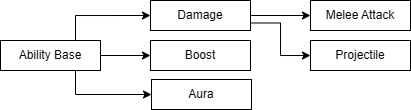
\includegraphics[width=0.75\linewidth]{obrazky-figures/spell-system.png}
    \caption{Vizualizácia tried ktoré tvoria systém schopností}
    \label{fig:spell-sys}
\end{figure}

\subsection{Nepriatelia}

Nepriatelia sa navigujú prostredím pomocou kontextového riadenia. Majú pevne daný okruh na detekovanie hráča no aby ho začali aktívne prenasledovať, musí medzi nimi byť neprerušený lúč, ktorý sa zastaví aj na stenách mapy. Po objavení hráča ho začne nepriateľ prenasledovať až do prerušenia kontaktu, ktorý vznikne napríklad zájdením za roh. V takom prípade si nepriateľ zapamätá a príde na posledné miesto na ktorom hráča videl.

V scéne sa nachádza aj objekt zodpovedný za pathfinding. Každý nepriateľ ktorý môže hliadkovať ho pri vytvorení vyhľadá a vypýta si hliadkovaciu trasu. Táto trasa sa získa pomocou JPS algoritmu, v ktorom sa do cesty uložia body v ktorých sa mení smer. Pri implementácii JPS algoritmu sme sa inšpirovali článkom \footnote{Článok JPS algoritmus - \url{https://zerowidth.com/2013/}}. A vychádza z našej implementácie A* algoritmu, pri ktorom využívame ako heuristiku Euklidskú vzdialenosť. Nepriatelia sa po tejto ceste pohybujú až do konca, pričom stále využívajú kontextové riadenie. Na konci cesty sa poradie bodov vymení a oni pokračujú v hliadkovaní. Ak počas svojej cesty detekujú hráča, začnú ho prenasledovať. Ak ho stratia s dohľadu, vypýtajú si novú cestu, tentokrát zo začiatkom v poslednom známom mieste hráča. Hliadkovanie je súčasťou každého nepriateľa a je možné ho zapnúť podľa potreby. V hre sa nachádzajú $4$ typy nepriateľov z toho $2$ bossovia (viď obr. \ref{fig:enemies}), ktorý používajú silnejšiu verziu útokov.

\begin{figure} [H]
    \centering
    
\includegraphics[width=0.55\linewidth]{obrazky-figures/enemy-types.png}
    \caption{Ukážka grafiky nepriateľov, bežný nepriatelia vľavo, bossovia vpravo}
    \label{fig:enemies}
\end{figure}

\begin{figure} [H]
    \centering
    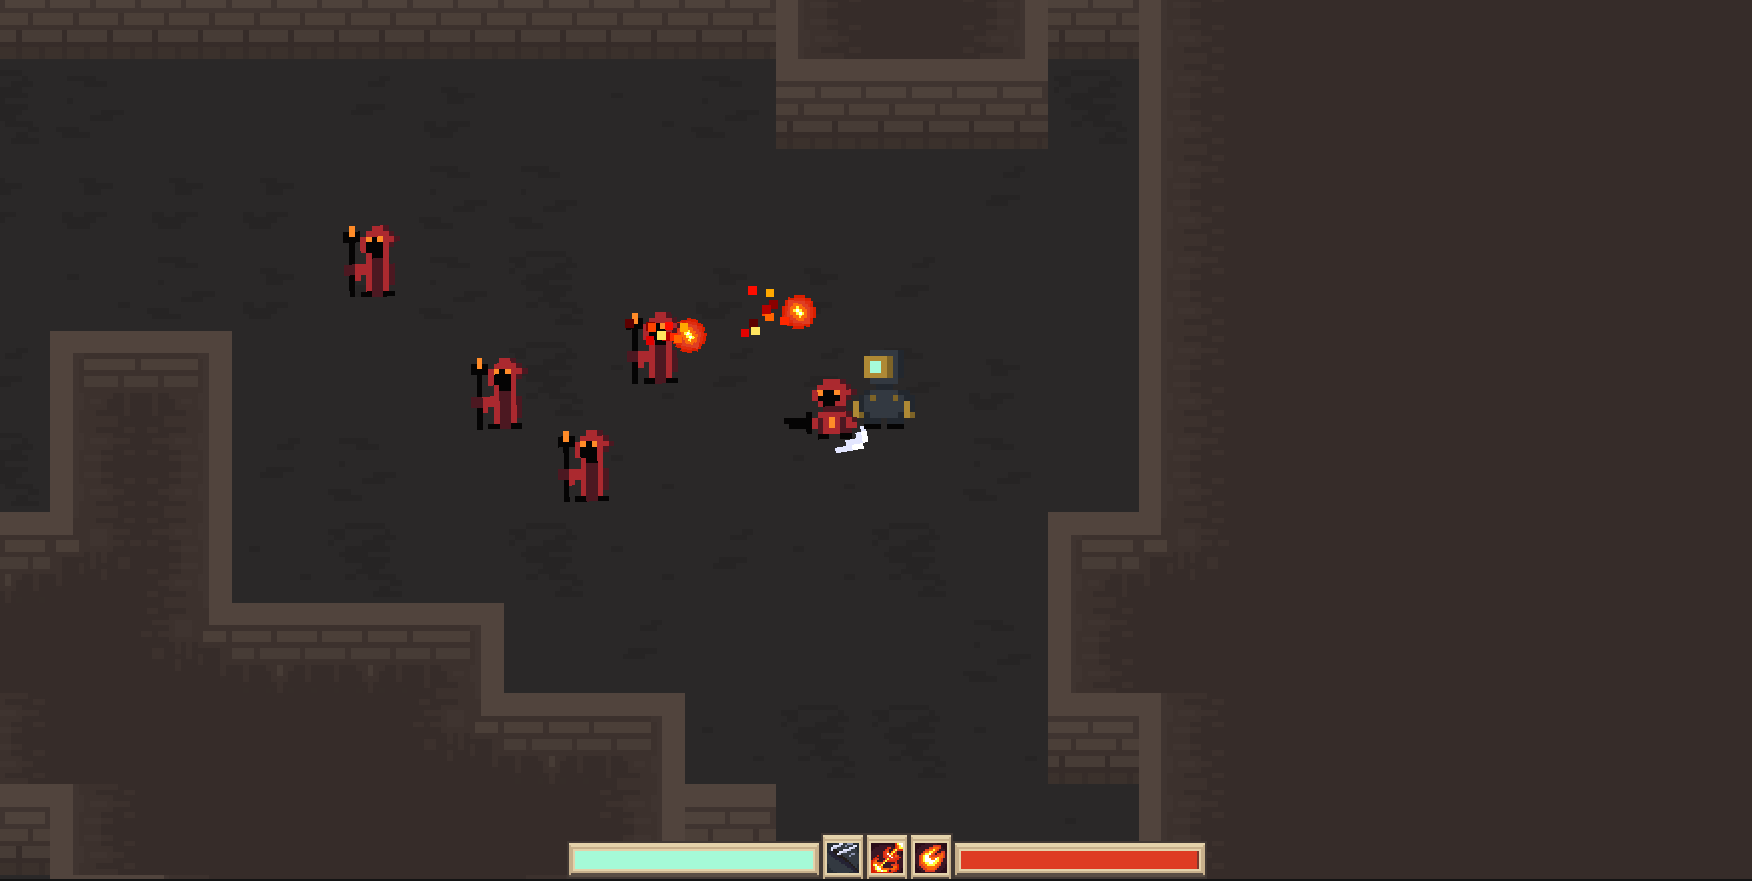
\includegraphics[width=1\linewidth]{obrazky-figures/screen.png}
    \caption{Ukážka finálnej verzie hry}
    \label{fig:screens}
\end{figure}

\chapter{Záver}

Vznik technológie procedurálneho generovania obsahu sprístupnil vývoj hier menším štúdiám tým, že odstránil potrebu veľkých tímov na tvorbu máp a herného sveta, ktoré sa zvyčajne spájajú s veľkými štúdiami a vysokými rozpočtami.

V súčasnom hernom prostredí je najdôležitejšie hráčov vtiahnuť do zábavnej hernej smičky a PCG zohráva hlavnú úlohu pri zvyšovaní rozmanitosti a nepredvídateľnosti v hrách. Čím poskytuje jedinečný herný zážitok pri každej iterácii a výrazne zvyšuje hodnotu hry a chuť hráčov si ju opätovne zahrať.

Okrem toho PCG slúži ako účinný nástroj na optimalizáciu zdrojov pri vývoji hier. Tradičné metódy tvorby obsahu často vyžadujú značné náklady na ľudský kapiták a časovú náročnosť, najmä pri ručnom vytváraní zložitých úrovní a prostredí. V našej práci sme implementovali iba základnú časť týchto metód a vidíme veľa možností na zlepšenie. Využitím algoritmov na generovanie obsahu a automatizáciou niektorých procesov návrhu sme schopný generovať prakticky nekonečné množstvo máp pre našu hru.

Z hľadiska hráča generovanie seedom dáva dôvod hráčom hľadať fóra a hernú komunitu, s cieľom získania zaujímavých máp. Takéto fóra môžeme považovať za virtuálnu databázu máp, ktorú môžu hráči rozširovať.

Hlavným cieľom tejto práce bolo dôkladné preskúmanie metodík PCG, najmä tých, ktoré sa vzťahujú na generovanie 2D máp vo videohrách. Prostredníctvom analýzy a porovnávania rôznych techník sme zistili ich výhody a najlepšie využitie. Implementovali sme ich do demonštračného prototypu hry tak, aby sme využili čo najlepšie ich potenciál a zistili, ktoré techniky sú vhodné na generovanie 2D terénu a naopak, ktoré nie. Ukážka vizuálnej stránky hry je na obr. \ref{fig:screens}. 

V súhrne naša práca zdôrazňuje nezastupiteľnú úlohu PCG pri formovaní súčasného prostredia vývoja videohier. Keďže technológie naďalej napredujú a tvorivé hranice sa rozširujú, PCG zostáva základným kameňom inovácií, ktorý uľahčuje vytváranie veľkého množstva obsahu malým vývojárom.